\documentclass[twoside]{book}

% Packages required by doxygen
\usepackage{fixltx2e}
\usepackage{calc}
\usepackage{doxygen}
\usepackage[export]{adjustbox} % also loads graphicx
\usepackage{graphicx}
\usepackage[utf8]{inputenc}
\usepackage{makeidx}
\usepackage{multicol}
\usepackage{multirow}
\PassOptionsToPackage{warn}{textcomp}
\usepackage{textcomp}
\usepackage[nointegrals]{wasysym}
\usepackage[table]{xcolor}

% Font selection
\usepackage[T1]{fontenc}
\usepackage[scaled=.90]{helvet}
\usepackage{courier}
\usepackage{amssymb}
\usepackage{sectsty}
\renewcommand{\familydefault}{\sfdefault}
\allsectionsfont{%
  \fontseries{bc}\selectfont%
  \color{darkgray}%
}
\renewcommand{\DoxyLabelFont}{%
  \fontseries{bc}\selectfont%
  \color{darkgray}%
}
\newcommand{\+}{\discretionary{\mbox{\scriptsize$\hookleftarrow$}}{}{}}

% Page & text layout
\usepackage{geometry}
\geometry{%
  a4paper,%
  top=2.5cm,%
  bottom=2.5cm,%
  left=2.5cm,%
  right=2.5cm%
}
\tolerance=750
\hfuzz=15pt
\hbadness=750
\setlength{\emergencystretch}{15pt}
\setlength{\parindent}{0cm}
\setlength{\parskip}{3ex plus 2ex minus 2ex}
\makeatletter
\renewcommand{\paragraph}{%
  \@startsection{paragraph}{4}{0ex}{-1.0ex}{1.0ex}{%
    \normalfont\normalsize\bfseries\SS@parafont%
  }%
}
\renewcommand{\subparagraph}{%
  \@startsection{subparagraph}{5}{0ex}{-1.0ex}{1.0ex}{%
    \normalfont\normalsize\bfseries\SS@subparafont%
  }%
}
\makeatother

% Headers & footers
\usepackage{fancyhdr}
\pagestyle{fancyplain}
\fancyhead[LE]{\fancyplain{}{\bfseries\thepage}}
\fancyhead[CE]{\fancyplain{}{}}
\fancyhead[RE]{\fancyplain{}{\bfseries\leftmark}}
\fancyhead[LO]{\fancyplain{}{\bfseries\rightmark}}
\fancyhead[CO]{\fancyplain{}{}}
\fancyhead[RO]{\fancyplain{}{\bfseries\thepage}}
\fancyfoot[LE]{\fancyplain{}{}}
\fancyfoot[CE]{\fancyplain{}{}}
\fancyfoot[RE]{\fancyplain{}{\bfseries\scriptsize Generated by Doxygen }}
\fancyfoot[LO]{\fancyplain{}{\bfseries\scriptsize Generated by Doxygen }}
\fancyfoot[CO]{\fancyplain{}{}}
\fancyfoot[RO]{\fancyplain{}{}}
\renewcommand{\footrulewidth}{0.4pt}
\renewcommand{\chaptermark}[1]{%
  \markboth{#1}{}%
}
\renewcommand{\sectionmark}[1]{%
  \markright{\thesection\ #1}%
}

% Indices & bibliography
\usepackage{natbib}
\usepackage[titles]{tocloft}
\setcounter{tocdepth}{3}
\setcounter{secnumdepth}{5}
\makeindex

% Hyperlinks (required, but should be loaded last)
\usepackage{ifpdf}
\ifpdf
  \usepackage[pdftex,pagebackref=true]{hyperref}
\else
  \usepackage[ps2pdf,pagebackref=true]{hyperref}
\fi
\hypersetup{%
  colorlinks=true,%
  linkcolor=blue,%
  citecolor=blue,%
  unicode%
}

% Custom commands
\newcommand{\clearemptydoublepage}{%
  \newpage{\pagestyle{empty}\cleardoublepage}%
}

\usepackage{caption}
\captionsetup{labelsep=space,justification=centering,font={bf},singlelinecheck=off,skip=4pt,position=top}

%===== C O N T E N T S =====

\begin{document}

% Titlepage & ToC
\hypersetup{pageanchor=false,
             bookmarksnumbered=true,
             pdfencoding=unicode
            }
\pagenumbering{roman}
\begin{titlepage}
\vspace*{7cm}
\begin{center}%
{\Large Dual Degree Project }\\
\vspace*{1cm}
{\large Generated by Doxygen 1.8.11}\\
\end{center}
\end{titlepage}
\clearemptydoublepage
\tableofcontents
\clearemptydoublepage
\pagenumbering{arabic}
\hypersetup{pageanchor=true}

%--- Begin generated contents ---
\chapter{My Personal Index Page}
\label{index}\hypertarget{index}{}\hypertarget{index_intro_sec}{}\section{Introduction}\label{index_intro_sec}
This is the C++ code to solve the high speed fluid flow. Currently, Euler flow is being solved but this code has been designed in moulder way so to solve the viscus flow additional viscus flux class can be added very easily. This code has been written to fulfill the requirement of the Dual Degree Project(\+D\+D\+P).\hypertarget{index_install_sec}{}\section{Installation \& Use}\label{index_install_sec}
To use the solver. Follow these simple steps.
\begin{DoxyItemize}
\item Download form here \+: \href{https://github.com/singh-kuldeep/DDP2}{\tt https\+://github.\+com/singh-\/kuldeep/\+D\+D\+P2} or \href{https://github.com/singh-kuldeep/DDP2}{\tt click here}
\item Go to the folder D\+D\+P2 and compile and run the file \hyperlink{TVD_8cpp}{T\+V\+D.\+cpp} (ex. g++ \hyperlink{TVD_8cpp}{T\+V\+D.\+cpp} \&\& ./a.out)
\item Nozzle has been set up as a default geometry but it can be changed from \char`\"{}run.\+h\char`\"{} file by uncommenting the header file
\item Currently there are two different geometry options are available
\begin{DoxyEnumerate}
\item Curved wall high area ratio diverging nozzle
\item Triangular bump inside straight duct
\end{DoxyEnumerate}
\end{DoxyItemize}\hypertarget{index_brief}{}\section{Brief about the solver}\label{index_brief}

\begin{DoxyItemize}
\item 3D Cartesian (x,y,z)
\item Roe scheme based
\item C++
\item Exact theory can be found \href{https://drive.google.com/open?id=0B9x_nh0D_HhzMnBjc0w5MmJpcnc}{\tt here}
\end{DoxyItemize}\hypertarget{index_input}{}\section{Input to the solver}\label{index_input}

\begin{DoxyItemize}
\item Grid points
\item Boundary condition
\item Some initial condition 
\end{DoxyItemize}\hypertarget{index_output}{}\section{Output files.}\label{index_output}
Here are the list of files which will come as the output of the solver.
\begin{DoxyItemize}
\item Residual\+\_\+\+Nozzle.\+csv \+: This file contains the all the residuals (Mass, Momentum, Energy).
\item grids\+\_\+\+Nozzle\+\_\+2\+D.\+csv \+: This file contains the grid point (x,y) coordinates.
\item 2\+D\+\_\+parameters\+\_\+\+B.\+csv \+: This file contains all the conserved parameters at the 2D plane. 
\end{DoxyItemize}\hypertarget{index_plot}{}\section{Results \& Plots}\label{index_plot}
Same older contains the M\+A\+T\+L\+AB script \char`\"{}plot\+\_\+data.\+m\char`\"{}. Once the simulation has started and the output files are generated, one can simply run the M\+A\+T\+A\+LB script and can see the plots which are listed below.
\begin{DoxyItemize}
\item Density Residual
\item X Momentum Residual
\item Y Momentum Residual
\item Z Momentum Residual
\item Energy Residual
\item Mach Number
\item Density
\item Velocity
\item Temperature
\item Pressure
\item Geometry 2D cross section 
\end{DoxyItemize}
\chapter{Bug List}
\label{bug}
\hypertarget{bug}{}

\begin{DoxyRefList}
\item[\label{bug__bug000001}%
\hypertarget{bug__bug000001}{}%
Member \hyperlink{classdiffusionfluxinterface_a30feb61f31b2c40063fc4ca7ca16258e}{diffusionfluxinterface\+:\+:diffusionfluxinterface} (vector$<$ double $>$ \&Conserved\+Variable\+Left\+Minus, vector$<$ double $>$ \&Conserved\+Variable\+Left, vector$<$ double $>$ \&Conserved\+Variable\+Right, vector$<$ double $>$ \&Conserved\+Variable\+Right\+Plus, vector$<$ double $>$ \&Face\+Area\+Vector\+Left, vector$<$ double $>$ \&Face\+Area\+Vector\+Right, vector$<$ double $>$ \&Face\+Area\+Vector\+Right\+Plus, double Cell\+Volume\+Left\+Mins, double Cell\+Volume\+Left, double Cell\+Volume\+Right, double Cell\+Volume\+Right\+Plus, double DeltaT)]Here syntax needs to be changed for gvactor\mbox{[}i\mbox{]} calculation 

Here I have doubt about \char`\"{}not equal to sign\char`\"{} because it can\textquotesingle{}t be exactly equal to 0.\+00000 so most of the time we end up choosing theta i = 0.\+0  
\item[\label{bug__bug000003}%
\hypertarget{bug__bug000003}{}%
File \hyperlink{dt_8h}{dt.h} ]Currently not using this, because \hyperlink{grid__nozzle_8h_a6cdf5cf168063009e847db46d6624c1b}{grid()} is not calculating ds value. So recheck this function as well after fixing the \hyperlink{grid__nozzle_8h_a6cdf5cf168063009e847db46d6624c1b}{grid()} function.  
\item[\label{bug__bug000004}%
\hypertarget{bug__bug000004}{}%
File \hyperlink{eulerflux_8h}{eulerflux.h} ]Not all memory is freed when deleting an object of this class.  
\item[\label{bug__bug000005}%
\hypertarget{bug__bug000005}{}%
Member \hyperlink{run_8h_ac7609273a01eb63ff8a25ddf1aafeff7}{grid} (vector$<$ vector$<$ vector$<$ vector$<$ double $>$ $>$ $>$ $>$ \&i\+Face\+Area\+Vector, vector$<$ vector$<$ vector$<$ vector$<$ double $>$ $>$ $>$ $>$ \&j\+Face\+Area\+Vector, vector$<$ vector$<$ vector$<$ vector$<$ double $>$ $>$ $>$ $>$ \&k\+Face\+Area\+Vector, vector$<$ vector$<$ vector$<$ double $>$ $>$ $>$ \&Cell\+Volume, vector$<$ vector$<$ vector$<$ double $>$ $>$ $>$ \&delta\+\_\+s, int \&Ni, int \&Nj, int \&Nk)]Yet to calculate the ds value properly  
\item[\label{bug__bug000005}%
\hypertarget{bug__bug000005}{}%
Member \hyperlink{run_8h_ac7609273a01eb63ff8a25ddf1aafeff7}{grid} (vector$<$ vector$<$ vector$<$ vector$<$ double $>$ $>$ $>$ $>$ \&i\+Face\+Area\+Vector, vector$<$ vector$<$ vector$<$ vector$<$ double $>$ $>$ $>$ $>$ \&j\+Face\+Area\+Vector, vector$<$ vector$<$ vector$<$ vector$<$ double $>$ $>$ $>$ $>$ \&k\+Face\+Area\+Vector, vector$<$ vector$<$ vector$<$ double $>$ $>$ $>$ \&Cell\+Volume, vector$<$ vector$<$ vector$<$ double $>$ $>$ $>$ \&delta\+\_\+s, int \&Ni, int \&Nj, int \&Nk)]Yet to calculate the ds value properly  
\item[\label{bug__bug000006}%
\hypertarget{bug__bug000006}{}%
Member \hyperlink{run_8h_a13a43e6d814de94978c515cb084873b1}{run} ()]Every time simulation starts from first iteration. So, to save the simulation it is good to start from the last solution as the initial condition 

Local time step needs to be used to reduce the simulation time 
\end{DoxyRefList}
\chapter{Class Index}
\section{Class List}
Here are the classes, structs, unions and interfaces with brief descriptions\+:\begin{DoxyCompactList}
\item\contentsline{section}{\hyperlink{classdiffusionfluxAUSM}{diffusionflux\+A\+U\+SM} }{\pageref{classdiffusionfluxAUSM}}{}
\item\contentsline{section}{\hyperlink{classdiffusionfluxinterface}{diffusionfluxinterface} }{\pageref{classdiffusionfluxinterface}}{}
\item\contentsline{section}{\hyperlink{classeulerflux}{eulerflux} }{\pageref{classeulerflux}}{}
\item\contentsline{section}{\hyperlink{classeulerfluxAUSM}{eulerflux\+A\+U\+SM} }{\pageref{classeulerfluxAUSM}}{}
\item\contentsline{section}{\hyperlink{classinterface}{interface} }{\pageref{classinterface}}{}
\item\contentsline{section}{\hyperlink{classnetfluxAUSM}{netflux\+A\+U\+SM} }{\pageref{classnetfluxAUSM}}{}
\item\contentsline{section}{\hyperlink{structnetfluxBase}{netflux\+Base} }{\pageref{structnetfluxBase}}{}
\item\contentsline{section}{\hyperlink{classnetfluxRoe}{netflux\+Roe} }{\pageref{classnetfluxRoe}}{}
\end{DoxyCompactList}

\chapter{File Index}
\section{File List}
Here is a list of all documented files with brief descriptions\+:\begin{DoxyCompactList}
\item\contentsline{section}{\hyperlink{BC_8h}{B\+C.\+h} \\*This header file implements all three boundary conditions }{\pageref{BC_8h}}{}
\item\contentsline{section}{\hyperlink{diffusionfluxinterface_8h}{diffusionfluxinterface.\+h} \\*This class calculates the numerical diffusion flux }{\pageref{diffusionfluxinterface_8h}}{}
\item\contentsline{section}{\hyperlink{dt_8h}{dt.\+h} \\*This header file conditions the function Time\+Step() which calculate the local time step for each cell at every iteration }{\pageref{dt_8h}}{}
\item\contentsline{section}{\hyperlink{eulerflux_8h}{eulerflux.\+h} \\*This class calculates the euler flux vectors(\+Ee,\+Fe,\+Ge) at the interface }{\pageref{eulerflux_8h}}{}
\item\contentsline{section}{{\bfseries grid\+\_\+diverging\+\_\+duct.\+h} }{\pageref{grid__diverging__duct_8h}}{}
\item\contentsline{section}{\hyperlink{grid__nozzle_8h}{grid\+\_\+nozzle.\+h} \\*This header file functions find the grid points, cell area vectors and the cell volumes }{\pageref{grid__nozzle_8h}}{}
\item\contentsline{section}{\hyperlink{interface_8h}{interface.\+h} \\*This class calculates the interface parameters using Reo scheme flux }{\pageref{interface_8h}}{}
\item\contentsline{section}{\hyperlink{netfluxinterface_8h}{netfluxinterface.\+h} \\*Calculates the net flux vector(numerical diffusion and euler flux) at the interface }{\pageref{netfluxinterface_8h}}{}
\item\contentsline{section}{\hyperlink{run_8h}{run.\+h} \\*This header file contains the \hyperlink{run_8h_a13a43e6d814de94978c515cb084873b1}{run()} function which runs the solver }{\pageref{run_8h}}{}
\end{DoxyCompactList}

\chapter{Class Documentation}
\hypertarget{classdiffusionfluxinterface}{}\section{diffusionfluxinterface Class Reference}
\label{classdiffusionfluxinterface}\index{diffusionfluxinterface@{diffusionfluxinterface}}
\subsection*{Public Member Functions}
\begin{DoxyCompactItemize}
\item 
\hyperlink{classdiffusionfluxinterface_a30feb61f31b2c40063fc4ca7ca16258e}{diffusionfluxinterface} (vector$<$ double $>$ \&Conserved\+Variable\+Left\+Minus, vector$<$ double $>$ \&Conserved\+Variable\+Left, vector$<$ double $>$ \&Conserved\+Variable\+Right, vector$<$ double $>$ \&Conserved\+Variable\+Right\+Plus, vector$<$ double $>$ \&Face\+Area\+Vector\+Left, vector$<$ double $>$ \&Face\+Area\+Vector\+Right, vector$<$ double $>$ \&Face\+Area\+Vector\+Right\+Plus, double Cell\+Volume\+Left\+Mins, double Cell\+Volume\+Left, double Cell\+Volume\+Right, double Cell\+Volume\+Right\+Plus, double DeltaT)
\end{DoxyCompactItemize}
\subsection*{Public Attributes}
\begin{DoxyCompactItemize}
\item 
double {\bfseries Diffusion\+Flux\+Vector} \mbox{[}5\mbox{]}\hypertarget{classdiffusionfluxinterface_a2e1da15c8bd0876ddb087c5cab930a28}{}\label{classdiffusionfluxinterface_a2e1da15c8bd0876ddb087c5cab930a28}

\end{DoxyCompactItemize}


\subsection{Constructor \& Destructor Documentation}
\index{diffusionfluxinterface@{diffusionfluxinterface}!diffusionfluxinterface@{diffusionfluxinterface}}
\index{diffusionfluxinterface@{diffusionfluxinterface}!diffusionfluxinterface@{diffusionfluxinterface}}
\subsubsection[{\texorpdfstring{diffusionfluxinterface(vector$<$ double $>$ \&\+Conserved\+Variable\+Left\+Minus, vector$<$ double $>$ \&\+Conserved\+Variable\+Left, vector$<$ double $>$ \&\+Conserved\+Variable\+Right, vector$<$ double $>$ \&\+Conserved\+Variable\+Right\+Plus, vector$<$ double $>$ \&\+Face\+Area\+Vector\+Left, vector$<$ double $>$ \&\+Face\+Area\+Vector\+Right, vector$<$ double $>$ \&\+Face\+Area\+Vector\+Right\+Plus, double Cell\+Volume\+Left\+Mins, double Cell\+Volume\+Left, double Cell\+Volume\+Right, double Cell\+Volume\+Right\+Plus, double Delta\+T)}{diffusionfluxinterface(vector< double > &ConservedVariableLeftMinus, vector< double > &ConservedVariableLeft, vector< double > &ConservedVariableRight, vector< double > &ConservedVariableRightPlus, vector< double > &FaceAreaVectorLeft, vector< double > &FaceAreaVectorRight, vector< double > &FaceAreaVectorRightPlus, double CellVolumeLeftMins, double CellVolumeLeft, double CellVolumeRight, double CellVolumeRightPlus, double DeltaT)}}]{\setlength{\rightskip}{0pt plus 5cm}diffusionfluxinterface\+::diffusionfluxinterface (
\begin{DoxyParamCaption}
\item[{vector$<$ double $>$ \&}]{Conserved\+Variable\+Left\+Minus, }
\item[{vector$<$ double $>$ \&}]{Conserved\+Variable\+Left, }
\item[{vector$<$ double $>$ \&}]{Conserved\+Variable\+Right, }
\item[{vector$<$ double $>$ \&}]{Conserved\+Variable\+Right\+Plus, }
\item[{vector$<$ double $>$ \&}]{Face\+Area\+Vector\+Left, }
\item[{vector$<$ double $>$ \&}]{Face\+Area\+Vector\+Right, }
\item[{vector$<$ double $>$ \&}]{Face\+Area\+Vector\+Right\+Plus, }
\item[{double}]{Cell\+Volume\+Left\+Mins, }
\item[{double}]{Cell\+Volume\+Left, }
\item[{double}]{Cell\+Volume\+Right, }
\item[{double}]{Cell\+Volume\+Right\+Plus, }
\item[{double}]{DeltaT}
\end{DoxyParamCaption}
)\hspace{0.3cm}{\ttfamily [inline]}}\hypertarget{classdiffusionfluxinterface_a30feb61f31b2c40063fc4ca7ca16258e}{}\label{classdiffusionfluxinterface_a30feb61f31b2c40063fc4ca7ca16258e}
\begin{DoxyRefDesc}{Bug}
\item[\hyperlink{bug__bug000002}{Bug}]Here syntax needs to be changed for gvactor\mbox{[}i\mbox{]} calculation \end{DoxyRefDesc}


\begin{DoxyRefDesc}{Bug}
\item[\hyperlink{bug__bug000003}{Bug}]Here I have doubt about \char`\"{}not equal to sign\char`\"{} because it can\textquotesingle{}t be exactly equal to 0.\+00000 so most of the time we end up choosing theta i = 0.\+0 \end{DoxyRefDesc}


The documentation for this class was generated from the following file\+:\begin{DoxyCompactItemize}
\item 
\hyperlink{diffusionfluxinterface_8h}{diffusionfluxinterface.\+h}\end{DoxyCompactItemize}

\hypertarget{classeulerflux}{}\section{eulerflux Class Reference}
\label{classeulerflux}\index{eulerflux@{eulerflux}}
\subsection*{Public Member Functions}
\begin{DoxyCompactItemize}
\item 
\hyperlink{classeulerflux_a184f13dbf2a62b11c443688049c1f4db}{eulerflux} (vector$<$ double $>$ \&Conserved\+Variable)
\end{DoxyCompactItemize}
\subsection*{Public Attributes}
\begin{DoxyCompactItemize}
\item 
double {\bfseries Euler\+FluxX} \mbox{[}5\mbox{]}\hypertarget{classeulerflux_a0282624fae997ac54441271130497185}{}\label{classeulerflux_a0282624fae997ac54441271130497185}

\item 
double {\bfseries Euler\+FluxY} \mbox{[}5\mbox{]}\hypertarget{classeulerflux_afdebc952e09629e73d7dcdda3e9e60ce}{}\label{classeulerflux_afdebc952e09629e73d7dcdda3e9e60ce}

\item 
double {\bfseries Euler\+FluxZ} \mbox{[}5\mbox{]}\hypertarget{classeulerflux_aaf2a28c94cb1cad57800342f8496c4b2}{}\label{classeulerflux_aaf2a28c94cb1cad57800342f8496c4b2}

\end{DoxyCompactItemize}


\subsection{Constructor \& Destructor Documentation}
\index{eulerflux@{eulerflux}!eulerflux@{eulerflux}}
\index{eulerflux@{eulerflux}!eulerflux@{eulerflux}}
\subsubsection[{\texorpdfstring{eulerflux(vector$<$ double $>$ \&\+Conserved\+Variable)}{eulerflux(vector< double > &ConservedVariable)}}]{\setlength{\rightskip}{0pt plus 5cm}eulerflux\+::eulerflux (
\begin{DoxyParamCaption}
\item[{vector$<$ double $>$ \&}]{Conserved\+Variable}
\end{DoxyParamCaption}
)\hspace{0.3cm}{\ttfamily [inline]}}\hypertarget{classeulerflux_a184f13dbf2a62b11c443688049c1f4db}{}\label{classeulerflux_a184f13dbf2a62b11c443688049c1f4db}

\begin{DoxyParams}[1]{Parameters}
 & {\em Euler\+FluxX} & x direction euler flux vector (Ee) at interface \\
\hline
 & {\em Euler\+FluxY} & y direction euler flux vector (Fe) at interface \\
\hline
 & {\em Euler\+FluxZ} & z direction euler flux vector (Ge) at interface \\
\hline
\mbox{\tt in}  & {\em Conserved\+Variable} & Conserved variable vector (\mbox{[}Density , x-\/momentum, y-\/momentum, z-\/momentum, Energy\mbox{]}) \\
\hline
 & {\em Pressure} & Satic pressure (p) \\
\hline
\end{DoxyParams}


The documentation for this class was generated from the following file\+:\begin{DoxyCompactItemize}
\item 
\hyperlink{eulerflux_8h}{eulerflux.\+h}\end{DoxyCompactItemize}

\hypertarget{classinterface}{}\section{interface Class Reference}
\label{classinterface}\index{interface@{interface}}
\subsection*{Public Member Functions}
\begin{DoxyCompactItemize}
\item 
{\bfseries interface} (vector$<$ double $>$ \&Conserved\+Variable\+Left, vector$<$ double $>$ \&Conserved\+Variable\+Right, vector$<$ double $>$ \&Face\+Area\+Vector\+Interface, double Cell\+Volume\+Left, double Cell\+Volume\+Right, double DeltaT)\hypertarget{classinterface_a7abecc6e69fdb7b0dc3a4ad0abbe4f93}{}\label{classinterface_a7abecc6e69fdb7b0dc3a4ad0abbe4f93}

\end{DoxyCompactItemize}
\subsection*{Public Attributes}
\begin{DoxyCompactItemize}
\item 
double {\bfseries Density\+Interface}\hypertarget{classinterface_a5a0a592bdfe7f5987c2c4f4424fbccd9}{}\label{classinterface_a5a0a592bdfe7f5987c2c4f4424fbccd9}

\item 
double {\bfseries Velocity\+X\+Interface}\hypertarget{classinterface_afae6ebb7814474f2264759a14521f448}{}\label{classinterface_afae6ebb7814474f2264759a14521f448}

\item 
double {\bfseries Velocity\+Y\+Interface}\hypertarget{classinterface_a0f42e6e3fd259e9fc191a255a6650ef6}{}\label{classinterface_a0f42e6e3fd259e9fc191a255a6650ef6}

\item 
double {\bfseries Velocity\+Z\+Interface}\hypertarget{classinterface_a1f1cc4570519d23fc38414472d7721f9}{}\label{classinterface_a1f1cc4570519d23fc38414472d7721f9}

\item 
double {\bfseries Enthalpy\+Interface}\hypertarget{classinterface_af2f6d43336396abc20bd88521e489a71}{}\label{classinterface_af2f6d43336396abc20bd88521e489a71}

\item 
double {\bfseries Vector\+Jump\+Interface} \mbox{[}5\mbox{]}\hypertarget{classinterface_aa99760e0d73f30c6f1541414efc76f87}{}\label{classinterface_aa99760e0d73f30c6f1541414efc76f87}

\item 
double {\bfseries Eigen\+Value} \mbox{[}5\mbox{]}\hypertarget{classinterface_a6e63abc816f019315477dc514963c505}{}\label{classinterface_a6e63abc816f019315477dc514963c505}

\item 
double {\bfseries Eigen\+Vector\+Matrix} \mbox{[}5\mbox{]}\mbox{[}5\mbox{]}\hypertarget{classinterface_a5889dedb2a24917fa46bd4c6515a33c7}{}\label{classinterface_a5889dedb2a24917fa46bd4c6515a33c7}

\item 
double {\bfseries Eigen\+Vector\+Matrix\+Inverse} \mbox{[}5\mbox{]}\mbox{[}5\mbox{]}\hypertarget{classinterface_ae67dd839deeeacfb620b114c560ea0a5}{}\label{classinterface_ae67dd839deeeacfb620b114c560ea0a5}

\item 
double {\bfseries Alpha\+Vector\+Interface} \mbox{[}5\mbox{]}\hypertarget{classinterface_aa3f54ad5bd8d3081383f2190090b4109}{}\label{classinterface_aa3f54ad5bd8d3081383f2190090b4109}

\item 
double {\bfseries Mu\+Vector\+Interface} \mbox{[}5\mbox{]}\hypertarget{classinterface_aa740f1171fcddcb604c237cabbcebc1a}{}\label{classinterface_aa740f1171fcddcb604c237cabbcebc1a}

\item 
double {\bfseries Z\+Vector\+Interface} \mbox{[}5\mbox{]}\hypertarget{classinterface_a32902e62056c2479ade3f78167f1522f}{}\label{classinterface_a32902e62056c2479ade3f78167f1522f}

\item 
double {\bfseries Pshi\+Vector\+Interface} \mbox{[}5\mbox{]}\hypertarget{classinterface_a37044e7a6a8820ea4bcbcaf969628238}{}\label{classinterface_a37044e7a6a8820ea4bcbcaf969628238}

\item 
double {\bfseries G\+Vector\+Interface} \mbox{[}5\mbox{]}\hypertarget{classinterface_ab25dbd2f7aaa6921fd5edb973af98ed4}{}\label{classinterface_ab25dbd2f7aaa6921fd5edb973af98ed4}

\end{DoxyCompactItemize}


The documentation for this class was generated from the following file\+:\begin{DoxyCompactItemize}
\item 
\hyperlink{interface_8h}{interface.\+h}\end{DoxyCompactItemize}

\hypertarget{classnetfluxinterface}{}\section{netfluxinterface Class Reference}
\label{classnetfluxinterface}\index{netfluxinterface@{netfluxinterface}}
\subsection*{Public Member Functions}
\begin{DoxyCompactItemize}
\item 
\hyperlink{classnetfluxinterface_aaa51271f4ed3cf28e7bf134cdb608589}{netfluxinterface} (vector$<$ double $>$ \&Conserved\+Variable\+Left\+Minus, vector$<$ double $>$ \&Conserved\+Variable\+Left, vector$<$ double $>$ \&Conserved\+Variable\+Right, vector$<$ double $>$ \&Conserved\+Variable\+Right\+Plus, vector$<$ double $>$ \&Face\+Area\+Left, vector$<$ double $>$ \&Face\+Area\+Vector\+Right, vector$<$ double $>$ \&Face\+Area\+Vector\+Rightplus, double Cell\+Volume\+Left\+Mins, double Cell\+Volume\+Left, double Cell\+Volume\+Right, double Cell\+Volume\+Right\+Plus, double DeltaT)
\end{DoxyCompactItemize}
\subsection*{Public Attributes}
\begin{DoxyCompactItemize}
\item 
double {\bfseries Net\+Flux} \mbox{[}5\mbox{]}\hypertarget{classnetfluxinterface_a32e1177d62968254eac419fd300c1208}{}\label{classnetfluxinterface_a32e1177d62968254eac419fd300c1208}

\end{DoxyCompactItemize}


\subsection{Constructor \& Destructor Documentation}
\index{netfluxinterface@{netfluxinterface}!netfluxinterface@{netfluxinterface}}
\index{netfluxinterface@{netfluxinterface}!netfluxinterface@{netfluxinterface}}
\subsubsection[{\texorpdfstring{netfluxinterface(vector$<$ double $>$ \&\+Conserved\+Variable\+Left\+Minus, vector$<$ double $>$ \&\+Conserved\+Variable\+Left, vector$<$ double $>$ \&\+Conserved\+Variable\+Right, vector$<$ double $>$ \&\+Conserved\+Variable\+Right\+Plus, vector$<$ double $>$ \&\+Face\+Area\+Left, vector$<$ double $>$ \&\+Face\+Area\+Vector\+Right, vector$<$ double $>$ \&\+Face\+Area\+Vector\+Rightplus, double Cell\+Volume\+Left\+Mins, double Cell\+Volume\+Left, double Cell\+Volume\+Right, double Cell\+Volume\+Right\+Plus, double Delta\+T)}{netfluxinterface(vector< double > &ConservedVariableLeftMinus, vector< double > &ConservedVariableLeft, vector< double > &ConservedVariableRight, vector< double > &ConservedVariableRightPlus, vector< double > &FaceAreaLeft, vector< double > &FaceAreaVectorRight, vector< double > &FaceAreaVectorRightplus, double CellVolumeLeftMins, double CellVolumeLeft, double CellVolumeRight, double CellVolumeRightPlus, double DeltaT)}}]{\setlength{\rightskip}{0pt plus 5cm}netfluxinterface\+::netfluxinterface (
\begin{DoxyParamCaption}
\item[{vector$<$ double $>$ \&}]{Conserved\+Variable\+Left\+Minus, }
\item[{vector$<$ double $>$ \&}]{Conserved\+Variable\+Left, }
\item[{vector$<$ double $>$ \&}]{Conserved\+Variable\+Right, }
\item[{vector$<$ double $>$ \&}]{Conserved\+Variable\+Right\+Plus, }
\item[{vector$<$ double $>$ \&}]{Face\+Area\+Left, }
\item[{vector$<$ double $>$ \&}]{Face\+Area\+Vector\+Right, }
\item[{vector$<$ double $>$ \&}]{Face\+Area\+Vector\+Rightplus, }
\item[{double}]{Cell\+Volume\+Left\+Mins, }
\item[{double}]{Cell\+Volume\+Left, }
\item[{double}]{Cell\+Volume\+Right, }
\item[{double}]{Cell\+Volume\+Right\+Plus, }
\item[{double}]{DeltaT}
\end{DoxyParamCaption}
)\hspace{0.3cm}{\ttfamily [inline]}}\hypertarget{classnetfluxinterface_aaa51271f4ed3cf28e7bf134cdb608589}{}\label{classnetfluxinterface_aaa51271f4ed3cf28e7bf134cdb608589}

\begin{DoxyParams}[1]{Parameters}
 & {\em Diffusion\+Flux\+Vector} & Numerical diffusion flux vector at the interface \\
\hline
\mbox{\tt in}  & {\em Conserved\+Variable} & Conserved variable vector (\mbox{[}Density , x-\/momentum, y-\/momentum, z-\/momentum, Energy\mbox{]}) \\
\hline
\mbox{\tt in}  & {\em Cell\+Vulume} & Pointer to the cell volume vector \\
\hline
\mbox{\tt in}  & {\em Left\+Minus} & Cell just previous to the left \\
\hline
\mbox{\tt in}  & {\em Right\+Plus} & Cell just Next to the right \\
\hline
\mbox{\tt in}  & {\em DeltaT} & Time step \\
\hline
\end{DoxyParams}

\begin{DoxyParams}{Parameters}
{\em left} & This object is euler flux calculated using the left cell conserved variables\\
\hline
{\em right} & This object is euler flux calculated using the right cell conserved variables\\
\hline
{\em Cell\+Volume\+Interface} & Average of left and right cell volume\\
\hline
\end{DoxyParams}
\begin{DoxySeeAlso}{See also}
\hyperlink{classdiffusionfluxinterface}{diffusionfluxinterface()} 

\hyperlink{classeulerflux}{eulerflux()}
\end{DoxySeeAlso}


The documentation for this class was generated from the following file\+:\begin{DoxyCompactItemize}
\item 
\hyperlink{netfluxinterface_8h}{netfluxinterface.\+h}\end{DoxyCompactItemize}

\chapter{File Documentation}
\hypertarget{BC_8h}{}\section{B\+C.\+h File Reference}
\label{BC_8h}\index{B\+C.\+h@{B\+C.\+h}}


A Documented file.  


{\ttfamily \#include \char`\"{}iostream\char`\"{}}\\*
{\ttfamily \#include \char`\"{}math.\+h\char`\"{}}\\*
{\ttfamily \#include $<$vector$>$}\\*
Include dependency graph for B\+C.\+h\+:

\hypertarget{diffusionfluxinterface_8h}{}\section{diffusionfluxinterface.\+h File Reference}
\label{diffusionfluxinterface_8h}\index{diffusionfluxinterface.\+h@{diffusionfluxinterface.\+h}}


This class calculates the numerical diffusion flux.  


{\ttfamily \#include \char`\"{}math.\+h\char`\"{}}\\*
{\ttfamily \#include \char`\"{}interface.\+h\char`\"{}}\\*
Include dependency graph for diffusionfluxinterface.\+h\+:\nopagebreak
\begin{figure}[H]
\begin{center}
\leavevmode
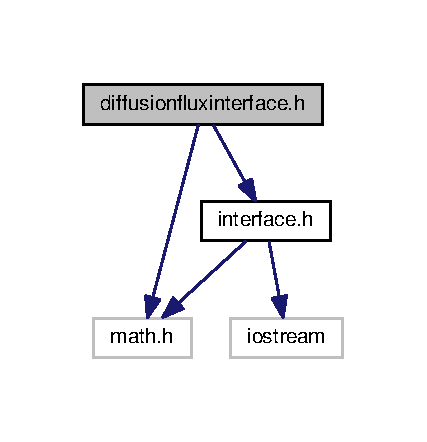
\includegraphics[width=205pt]{diffusionfluxinterface_8h__incl}
\end{center}
\end{figure}
This graph shows which files directly or indirectly include this file\+:
\nopagebreak
\begin{figure}[H]
\begin{center}
\leavevmode
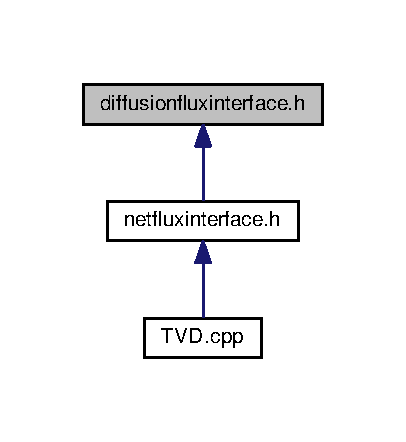
\includegraphics[width=199pt]{diffusionfluxinterface_8h__dep__incl}
\end{center}
\end{figure}
\subsection*{Classes}
\begin{DoxyCompactItemize}
\item 
class \hyperlink{classdiffusionfluxinterface}{diffusionfluxinterface}
\end{DoxyCompactItemize}


\subsection{Detailed Description}
This class calculates the numerical diffusion flux. 

\begin{DoxyAuthor}{Author}
Kuldeep Singh 
\end{DoxyAuthor}
\begin{DoxyDate}{Date}
2017 
\end{DoxyDate}
\begin{DoxyCopyright}{Copyright}
G\+NU Public License.
\end{DoxyCopyright}

\begin{DoxyParams}[1]{Parameters}
 & {\em Diffusion\+Flux\+Vector} & Numerical diffusion flux vector at the interface \\
\hline
\mbox{\tt in}  & {\em Conserved\+Variable} & Conserved variable vector (\mbox{[}Density , x-\/momentum, y-\/momentum, z-\/momentum, Energy\mbox{]}) \\
\hline
\mbox{\tt in}  & {\em Cell\+Vulume} & Pointer to the cell volume vector \\
\hline
\mbox{\tt in}  & {\em Left\+Minus} & Cell just previous to the left \\
\hline
\mbox{\tt in}  & {\em Right\+Plus} & Cell just Next to the right \\
\hline
\mbox{\tt in}  & {\em DeltaT} & Time step \\
\hline
\end{DoxyParams}
\begin{DoxyRefDesc}{Bug}
\item[\hyperlink{bug__bug000001}{Bug}]Needs to explain the code little bit more. \end{DoxyRefDesc}

\hypertarget{eulerflux_8h}{}\section{eulerflux.\+h File Reference}
\label{eulerflux_8h}\index{eulerflux.\+h@{eulerflux.\+h}}


This class calculates the euler flux vectors(\+Ee,\+Fe,\+Ge) at the interface.  


{\ttfamily \#include \char`\"{}math.\+h\char`\"{}}\\*
{\ttfamily \#include \char`\"{}iostream\char`\"{}}\\*
Include dependency graph for eulerflux.\+h\+:\nopagebreak
\begin{figure}[H]
\begin{center}
\leavevmode
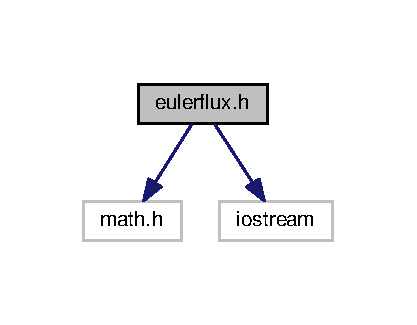
\includegraphics[width=200pt]{eulerflux_8h__incl}
\end{center}
\end{figure}
This graph shows which files directly or indirectly include this file\+:
\nopagebreak
\begin{figure}[H]
\begin{center}
\leavevmode
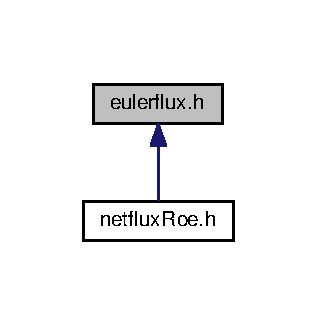
\includegraphics[width=172pt]{eulerflux_8h__dep__incl}
\end{center}
\end{figure}
\subsection*{Classes}
\begin{DoxyCompactItemize}
\item 
class \hyperlink{classeulerflux}{eulerflux}
\end{DoxyCompactItemize}
\subsection*{Macros}
\begin{DoxyCompactItemize}
\item 
\#define \hyperlink{eulerflux_8h_ab683b1fef77e9bd4205b818c943fec96}{Specific\+Heat\+Ratio}~1.\+4
\end{DoxyCompactItemize}


\subsection{Detailed Description}
This class calculates the euler flux vectors(\+Ee,\+Fe,\+Ge) at the interface. 

\begin{DoxyAuthor}{Author}
Kuldeep Singh 
\end{DoxyAuthor}
\begin{DoxyDate}{Date}
2017 
\end{DoxyDate}
\begin{DoxyRefDesc}{Bug}
\item[\hyperlink{bug__bug000004}{Bug}]Not all memory is freed when deleting an object of this class. \end{DoxyRefDesc}
\begin{DoxyCopyright}{Copyright}
G\+NU Public License. 
\end{DoxyCopyright}

\begin{DoxyParams}[1]{Parameters}
 & {\em Euler\+FluxX} & x direction euler flux vector (Ee) at interface \\
\hline
 & {\em Euler\+FluxY} & y direction euler flux vector (Fe) at interface \\
\hline
 & {\em Euler\+FluxZ} & z direction euler flux vector (Ge) at interface \\
\hline
\mbox{\tt in}  & {\em Conserved\+Variable} & Conserved variable vector (\mbox{[}Density , x-\/momentum, y-\/momentum, z-\/momentum, Energy\mbox{]}) \\
\hline
 & {\em Pressure} & Satic pressure (p) \\
\hline
\end{DoxyParams}


\subsection{Macro Definition Documentation}
\index{eulerflux.\+h@{eulerflux.\+h}!Specific\+Heat\+Ratio@{Specific\+Heat\+Ratio}}
\index{Specific\+Heat\+Ratio@{Specific\+Heat\+Ratio}!eulerflux.\+h@{eulerflux.\+h}}
\subsubsection[{\texorpdfstring{Specific\+Heat\+Ratio}{SpecificHeatRatio}}]{\setlength{\rightskip}{0pt plus 5cm}\#define Specific\+Heat\+Ratio~1.\+4}\hypertarget{eulerflux_8h_ab683b1fef77e9bd4205b818c943fec96}{}\label{eulerflux_8h_ab683b1fef77e9bd4205b818c943fec96}
This is gas constant (Gamma). For air at room temperature it is almost equal to 1.\+4. If you are using some other gas at some other temperature then change it 
\hypertarget{grid__ideal__nozzle_8h}{}\section{grid\+\_\+ideal\+\_\+nozzle.\+h File Reference}
\label{grid__ideal__nozzle_8h}\index{grid\+\_\+ideal\+\_\+nozzle.\+h@{grid\+\_\+ideal\+\_\+nozzle.\+h}}


This header file functions find the grid points, cell area vectors and the cell volumes for the ideal nozzle. In which nozzle has ans uniform flow at the exit. Because in the cancellation of expansion fan has been done by compression waves.  


{\ttfamily \#include $<$iostream$>$}\\*
{\ttfamily \#include \char`\"{}math.\+h\char`\"{}}\\*
{\ttfamily \#include $<$fstream$>$}\\*
{\ttfamily \#include $<$string$>$}\\*
{\ttfamily \#include $<$vector$>$}\\*
{\ttfamily \#include $<$cstdlib$>$}\\*
Include dependency graph for grid\+\_\+ideal\+\_\+nozzle.\+h\+:
\nopagebreak
\begin{figure}[H]
\begin{center}
\leavevmode
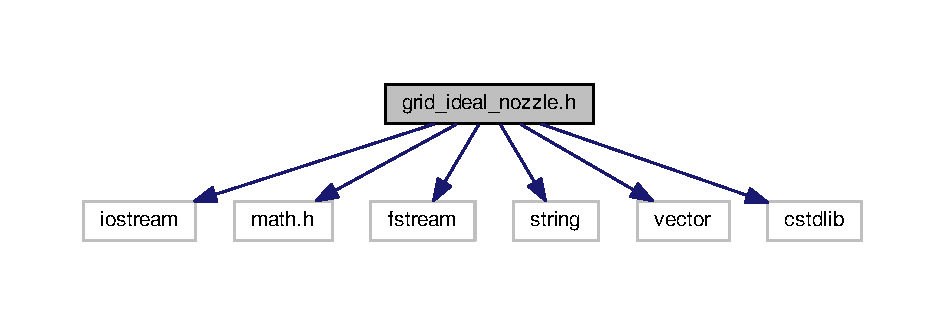
\includegraphics[width=350pt]{grid__ideal__nozzle_8h__incl}
\end{center}
\end{figure}
\subsection*{Functions}
\begin{DoxyCompactItemize}
\item 
double \hyperlink{grid__ideal__nozzle_8h_a49295397147e6ac59b00e1802fb652cf}{finddz} (std\+::vector$<$ std\+::vector$<$ double $>$ $>$ Down\+Coordinates)
\begin{DoxyCompactList}\small\item\em Find the cell side in z direction by taking average of all dx for dz. \end{DoxyCompactList}\item 
double \hyperlink{grid__ideal__nozzle_8h_adeaf7cb110880d4dc16735a6d3afdbf8}{distance} (std\+::vector$<$ double $>$ p1, std\+::vector$<$ double $>$ p2)
\begin{DoxyCompactList}\small\item\em Calculates the distance between the two points in 3D space. \end{DoxyCompactList}\item 
void \hyperlink{grid__ideal__nozzle_8h_a5864956dd2d7c0cd17af385ddab35597}{take\+Mirror} (double \&x, double \&y, double x1, double y1, double x2, double y2, double l, double m)
\begin{DoxyCompactList}\small\item\em This function will take boundary cell grid points and will calculate the ghost cell grid points by taking the mirror image about the boundary. \end{DoxyCompactList}\item 
void \hyperlink{grid__ideal__nozzle_8h_a0195a06d59a6445d9ef8d27b775caeb0}{grid} (vector$<$ vector$<$ vector$<$ vector$<$ double $>$ $>$ $>$ $>$ \&i\+Face\+Area\+Vector\+In, vector$<$ vector$<$ vector$<$ vector$<$ double $>$ $>$ $>$ $>$ \&j\+Face\+Area\+Vector\+In, vector$<$ vector$<$ vector$<$ vector$<$ double $>$ $>$ $>$ $>$ \&k\+Face\+Area\+Vector\+In, vector$<$ vector$<$ vector$<$ double $>$ $>$ $>$ \&Cell\+Volume\+In, vector$<$ vector$<$ vector$<$ double $>$ $>$ $>$ \&ds\+In, int \&Ni, int \&Nj, int \&Nk, int Geometry\+Option)
\begin{DoxyCompactList}\small\item\em This function calculates the cell area and the cell volumes of all cells including the ghost cells. \end{DoxyCompactList}\end{DoxyCompactItemize}


\subsection{Detailed Description}
This header file functions find the grid points, cell area vectors and the cell volumes for the ideal nozzle. In which nozzle has ans uniform flow at the exit. Because in the cancellation of expansion fan has been done by compression waves. 

\begin{DoxyAuthor}{Author}
Kuldeep Singh 
\end{DoxyAuthor}
\begin{DoxyDate}{Date}
2017 
\end{DoxyDate}
\begin{DoxyWarning}{Warning}
For different geometries change this file accordingly. 
\end{DoxyWarning}


\subsection{Function Documentation}
\index{grid\+\_\+ideal\+\_\+nozzle.\+h@{grid\+\_\+ideal\+\_\+nozzle.\+h}!distance@{distance}}
\index{distance@{distance}!grid\+\_\+ideal\+\_\+nozzle.\+h@{grid\+\_\+ideal\+\_\+nozzle.\+h}}
\subsubsection[{\texorpdfstring{distance(std\+::vector$<$ double $>$ p1, std\+::vector$<$ double $>$ p2)}{distance(std::vector< double > p1, std::vector< double > p2)}}]{\setlength{\rightskip}{0pt plus 5cm}double distance (
\begin{DoxyParamCaption}
\item[{std\+::vector$<$ double $>$}]{p1, }
\item[{std\+::vector$<$ double $>$}]{p2}
\end{DoxyParamCaption}
)}\hypertarget{grid__ideal__nozzle_8h_adeaf7cb110880d4dc16735a6d3afdbf8}{}\label{grid__ideal__nozzle_8h_adeaf7cb110880d4dc16735a6d3afdbf8}


Calculates the distance between the two points in 3D space. 


\begin{DoxyParams}[1]{Parameters}
\mbox{\tt in}  & {\em p1} & First point. \\
\hline
\mbox{\tt in}  & {\em p2} & Second point. \\
\hline
\end{DoxyParams}
\begin{DoxyReturn}{Returns}
Distance between the two points 
\end{DoxyReturn}
\index{grid\+\_\+ideal\+\_\+nozzle.\+h@{grid\+\_\+ideal\+\_\+nozzle.\+h}!finddz@{finddz}}
\index{finddz@{finddz}!grid\+\_\+ideal\+\_\+nozzle.\+h@{grid\+\_\+ideal\+\_\+nozzle.\+h}}
\subsubsection[{\texorpdfstring{finddz(std\+::vector$<$ std\+::vector$<$ double $>$ $>$ Down\+Coordinates)}{finddz(std::vector< std::vector< double > > DownCoordinates)}}]{\setlength{\rightskip}{0pt plus 5cm}double finddz (
\begin{DoxyParamCaption}
\item[{std\+::vector$<$ std\+::vector$<$ double $>$ $>$}]{Down\+Coordinates}
\end{DoxyParamCaption}
)}\hypertarget{grid__ideal__nozzle_8h_a49295397147e6ac59b00e1802fb652cf}{}\label{grid__ideal__nozzle_8h_a49295397147e6ac59b00e1802fb652cf}


Find the cell side in z direction by taking average of all dx for dz. 


\begin{DoxyParams}[1]{Parameters}
\mbox{\tt in}  & {\em Down\+Coordinates} & (x,y)coordinates of the down wall of the nozzle. \\
\hline
\end{DoxyParams}
\begin{DoxyReturn}{Returns}
double 
\end{DoxyReturn}
\index{grid\+\_\+ideal\+\_\+nozzle.\+h@{grid\+\_\+ideal\+\_\+nozzle.\+h}!grid@{grid}}
\index{grid@{grid}!grid\+\_\+ideal\+\_\+nozzle.\+h@{grid\+\_\+ideal\+\_\+nozzle.\+h}}
\subsubsection[{\texorpdfstring{grid(vector$<$ vector$<$ vector$<$ vector$<$ double $>$ $>$ $>$ $>$ \&i\+Face\+Area\+Vector\+In, vector$<$ vector$<$ vector$<$ vector$<$ double $>$ $>$ $>$ $>$ \&j\+Face\+Area\+Vector\+In, vector$<$ vector$<$ vector$<$ vector$<$ double $>$ $>$ $>$ $>$ \&k\+Face\+Area\+Vector\+In, vector$<$ vector$<$ vector$<$ double $>$ $>$ $>$ \&\+Cell\+Volume\+In, vector$<$ vector$<$ vector$<$ double $>$ $>$ $>$ \&ds\+In, int \&\+Ni, int \&\+Nj, int \&\+Nk, int Geometry\+Option)}{grid(vector< vector< vector< vector< double > > > > &iFaceAreaVectorIn, vector< vector< vector< vector< double > > > > &jFaceAreaVectorIn, vector< vector< vector< vector< double > > > > &kFaceAreaVectorIn, vector< vector< vector< double > > > &CellVolumeIn, vector< vector< vector< double > > > &dsIn, int &Ni, int &Nj, int &Nk, int GeometryOption)}}]{\setlength{\rightskip}{0pt plus 5cm}void grid (
\begin{DoxyParamCaption}
\item[{vector$<$ vector$<$ vector$<$ vector$<$ double $>$ $>$ $>$ $>$ \&}]{i\+Face\+Area\+Vector\+In, }
\item[{vector$<$ vector$<$ vector$<$ vector$<$ double $>$ $>$ $>$ $>$ \&}]{j\+Face\+Area\+Vector\+In, }
\item[{vector$<$ vector$<$ vector$<$ vector$<$ double $>$ $>$ $>$ $>$ \&}]{k\+Face\+Area\+Vector\+In, }
\item[{vector$<$ vector$<$ vector$<$ double $>$ $>$ $>$ \&}]{Cell\+Volume\+In, }
\item[{vector$<$ vector$<$ vector$<$ double $>$ $>$ $>$ \&}]{ds\+In, }
\item[{int \&}]{Ni, }
\item[{int \&}]{Nj, }
\item[{int \&}]{Nk, }
\item[{int}]{Geometry\+Option}
\end{DoxyParamCaption}
)}\hypertarget{grid__ideal__nozzle_8h_a0195a06d59a6445d9ef8d27b775caeb0}{}\label{grid__ideal__nozzle_8h_a0195a06d59a6445d9ef8d27b775caeb0}


This function calculates the cell area and the cell volumes of all cells including the ghost cells. 

This function generates the area vector and cell volumes inside the domain whole domain.


\begin{DoxyParams}[1]{Parameters}
\mbox{\tt in}  & {\em i\+Face\+Area\+Vector\+In} & Input pointer to \char`\"{}i\char`\"{} faces area vector \\
\hline
\mbox{\tt in}  & {\em j\+Face\+Area\+Vector\+In} & Input pointer to \char`\"{}j\char`\"{} faces area vector \\
\hline
\mbox{\tt in}  & {\em k\+Face\+Area\+Vector\+In} & Input pointer to \char`\"{}k\char`\"{} faces area vector \\
\hline
\mbox{\tt in}  & {\em Cell\+Volume\+In} & Input pointer to cell volumes \\
\hline
\mbox{\tt in}  & {\em ds\+In} & Input pointer to minimum distance \\
\hline
 & {\em Upper\+Coordinates} & Upper wall coordinates (x,y) of the nozzle geometry \\
\hline
 & {\em Down\+Coordinates} & Down wall coordinates (x,y) of the nozzle geometry \\
\hline
\end{DoxyParams}
\begin{DoxyReturn}{Returns}
void 
\end{DoxyReturn}

\begin{DoxyParams}[1]{Parameters}
 & {\em N} & Total cells in j direction\\
\hline
 & {\em N+1} & Total \char`\"{}grid points\char`\"{} in j direction after including the boundary points\\
\hline
\mbox{\tt in}  & {\em Ni} & Number of cells(\+Including ghost cells) in \char`\"{}i\char`\"{} direction.\\
\hline
\mbox{\tt in}  & {\em Nj} & Number of cells(\+Including ghost cells) in \char`\"{}j\char`\"{} direction.\\
\hline
\mbox{\tt in}  & {\em Nk} & Number of cells(\+Including ghost cells) in \char`\"{}k\char`\"{} direction.\\
\hline
 & {\em Coordinate} & 4D vector which stores the all coordinates of all cells (Including ghost) inside the domain\\
\hline
 & {\em i\+Face\+Area\+Vector} & 4D vector which stores the all \char`\"{}i\char`\"{} face area vectors of all cells(\+Including ghost) inside the domain\\
\hline
 & {\em j\+Face\+Area\+Vector} & 4D vector which stores the all \char`\"{}j\char`\"{} face area vectors of all cells(\+Including ghost) inside the domain\\
\hline
 & {\em k\+Face\+Area\+Vector} & 4D vector which stores the all \char`\"{}k\char`\"{} face area vectors of all cells(\+Including ghost) inside the domain\\
\hline
 & {\em Cell\+Volume} & 3D vector which stores the cell volume of all cells (Including ghost) inside the domain\\
\hline
 & {\em (x0,y0)} & Live cell coordinates which needs to be mirrored to get the ghost cell coordinates\\
\hline
 & {\em (x1,y1)} & Next live cell coordinates which needs to be mirrored to get the ghost cell coordinates\\
\hline
 & {\em (l0,m0),(l1,m1)} & Line about which reflection needs to be taken\\
\hline
 & {\em (rx0,ry0)} & Ghost cell grid point\\
\hline
 & {\em (rx1,ry1)} & Ghost cell next grid point\\
\hline
\end{DoxyParams}
Structure of grid out put file (\char`\"{}grids\+\_\+\+Nozzle\+\_\+2\+D.\+csv\char`\"{})
\begin{DoxyItemize}
\item First line of the grid file will contain grid points (excluding ghost cells) in x and y direction
\item This will exclude the ghost, only live cells or actual geomatry points
\end{DoxyItemize}\index{grid\+\_\+ideal\+\_\+nozzle.\+h@{grid\+\_\+ideal\+\_\+nozzle.\+h}!take\+Mirror@{take\+Mirror}}
\index{take\+Mirror@{take\+Mirror}!grid\+\_\+ideal\+\_\+nozzle.\+h@{grid\+\_\+ideal\+\_\+nozzle.\+h}}
\subsubsection[{\texorpdfstring{take\+Mirror(double \&x, double \&y, double x1, double y1, double x2, double y2, double l, double m)}{takeMirror(double &x, double &y, double x1, double y1, double x2, double y2, double l, double m)}}]{\setlength{\rightskip}{0pt plus 5cm}void take\+Mirror (
\begin{DoxyParamCaption}
\item[{double \&}]{x, }
\item[{double \&}]{y, }
\item[{double}]{x1, }
\item[{double}]{y1, }
\item[{double}]{x2, }
\item[{double}]{y2, }
\item[{double}]{l, }
\item[{double}]{m}
\end{DoxyParamCaption}
)}\hypertarget{grid__ideal__nozzle_8h_a5864956dd2d7c0cd17af385ddab35597}{}\label{grid__ideal__nozzle_8h_a5864956dd2d7c0cd17af385ddab35597}


This function will take boundary cell grid points and will calculate the ghost cell grid points by taking the mirror image about the boundary. 


\begin{DoxyParams}[1]{Parameters}
\mbox{\tt in}  & {\em \&x} & Pointer to x coordinate after taking mirror image \\
\hline
\mbox{\tt in}  & {\em \&y} & Pointer to y coordinate after taking mirror image \\
\hline
\mbox{\tt in}  & {\em l} & x coordinate of the point which is to mirrored \\
\hline
\mbox{\tt in}  & {\em m} & y coordinate of the point which is to mirrored \\
\hline
\mbox{\tt in}  & {\em (x1,y1)} & Starting point of the line about which mirror is taken \\
\hline
\mbox{\tt in}  & {\em (x2,y2)} & End point of the line about which mirror is taken \\
\hline
\end{DoxyParams}
\begin{DoxyReturn}{Returns}
void 
\end{DoxyReturn}

\hypertarget{grid__nozzle_8h}{}\section{grid\+\_\+nozzle.\+h File Reference}
\label{grid__nozzle_8h}\index{grid\+\_\+nozzle.\+h@{grid\+\_\+nozzle.\+h}}


This header file functions find the grid points, cell area vectors and the cell volumes. This is just a sample test case.  


{\ttfamily \#include $<$iostream$>$}\\*
{\ttfamily \#include \char`\"{}math.\+h\char`\"{}}\\*
{\ttfamily \#include $<$fstream$>$}\\*
{\ttfamily \#include $<$string$>$}\\*
{\ttfamily \#include $<$vector$>$}\\*
{\ttfamily \#include $<$cstdlib$>$}\\*
Include dependency graph for grid\+\_\+nozzle.\+h\+:\nopagebreak
\begin{figure}[H]
\begin{center}
\leavevmode
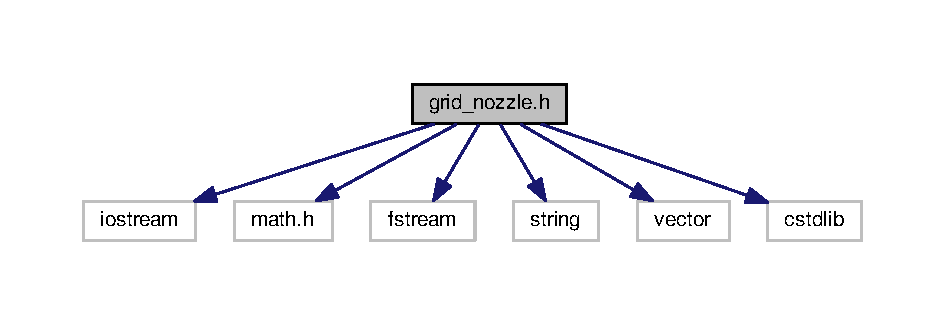
\includegraphics[width=350pt]{grid__nozzle_8h__incl}
\end{center}
\end{figure}
\subsection*{Functions}
\begin{DoxyCompactItemize}
\item 
double \hyperlink{grid__nozzle_8h_a7d60261a6b97e33ed453329ea74dcaeb}{findY} (double x, std\+::vector$<$ std\+::vector$<$ double $>$ $>$ Upper\+Coordinates)
\begin{DoxyCompactList}\small\item\em This function finds the value of the y coordinate of the upper wall at x. \end{DoxyCompactList}\item 
double \hyperlink{grid__nozzle_8h_a5095cfcdfa89a4f1571776aea37aabac}{finddz} (std\+::vector$<$ std\+::vector$<$ double $>$ $>$ Down\+Coordinates\+New)
\begin{DoxyCompactList}\small\item\em Find the cell side in z direction by taking average of all dx for dz. \end{DoxyCompactList}\item 
double \hyperlink{grid__nozzle_8h_adeaf7cb110880d4dc16735a6d3afdbf8}{distance} (std\+::vector$<$ double $>$ p1, std\+::vector$<$ double $>$ p2)
\begin{DoxyCompactList}\small\item\em Calculates the distance between the two points in 3D space. \end{DoxyCompactList}\item 
double \hyperlink{grid__nozzle_8h_a8e6462a9b7c30e3344fbce0766435913}{min} (double d1, double d2, double d3, double d4, double d5, double d6, double d7, double d8, double d9, double d10, double d11, double d12)
\begin{DoxyCompactList}\small\item\em Find the minimum out of the all input parameters. \end{DoxyCompactList}\item 
void \hyperlink{grid__nozzle_8h_a5864956dd2d7c0cd17af385ddab35597}{take\+Mirror} (double \&x, double \&y, double x1, double y1, double x2, double y2, double l, double m)
\begin{DoxyCompactList}\small\item\em This function will take boundary cell grid points and will calculate the ghost cell grid points by taking the mirror image about the boundary. \end{DoxyCompactList}\item 
void \hyperlink{grid__nozzle_8h_a6cdf5cf168063009e847db46d6624c1b}{grid} (vector$<$ vector$<$ vector$<$ vector$<$ double $>$ $>$ $>$ $>$ \&i\+Face\+Area\+Vector\+In, vector$<$ vector$<$ vector$<$ vector$<$ double $>$ $>$ $>$ $>$ \&j\+Face\+Area\+Vector\+In, vector$<$ vector$<$ vector$<$ vector$<$ double $>$ $>$ $>$ $>$ \&k\+Face\+Area\+Vector\+In, vector$<$ vector$<$ vector$<$ double $>$ $>$ $>$ \&Cell\+Volume\+In, vector$<$ vector$<$ vector$<$ double $>$ $>$ $>$ \&ds\+In, int \&Ni, int \&Nj, int \&Nk)
\begin{DoxyCompactList}\small\item\em This function calculates the cell area and the cell volumes of all cells including the ghost cells. \end{DoxyCompactList}\end{DoxyCompactItemize}


\subsection{Detailed Description}
This header file functions find the grid points, cell area vectors and the cell volumes. This is just a sample test case. 

\begin{DoxyAuthor}{Author}
Kuldeep Singh 
\end{DoxyAuthor}
\begin{DoxyDate}{Date}
2017 
\end{DoxyDate}
\begin{DoxyWarning}{Warning}
For different geometries change this file accordingly. 
\end{DoxyWarning}


\subsection{Function Documentation}
\index{grid\+\_\+nozzle.\+h@{grid\+\_\+nozzle.\+h}!distance@{distance}}
\index{distance@{distance}!grid\+\_\+nozzle.\+h@{grid\+\_\+nozzle.\+h}}
\subsubsection[{\texorpdfstring{distance(std\+::vector$<$ double $>$ p1, std\+::vector$<$ double $>$ p2)}{distance(std::vector< double > p1, std::vector< double > p2)}}]{\setlength{\rightskip}{0pt plus 5cm}double distance (
\begin{DoxyParamCaption}
\item[{std\+::vector$<$ double $>$}]{p1, }
\item[{std\+::vector$<$ double $>$}]{p2}
\end{DoxyParamCaption}
)}\hypertarget{grid__nozzle_8h_adeaf7cb110880d4dc16735a6d3afdbf8}{}\label{grid__nozzle_8h_adeaf7cb110880d4dc16735a6d3afdbf8}


Calculates the distance between the two points in 3D space. 


\begin{DoxyParams}[1]{Parameters}
\mbox{\tt in}  & {\em p1} & First point. \\
\hline
\mbox{\tt in}  & {\em p2} & Second point. \\
\hline
\end{DoxyParams}
\begin{DoxyReturn}{Returns}
Distance between the two points 
\end{DoxyReturn}
\index{grid\+\_\+nozzle.\+h@{grid\+\_\+nozzle.\+h}!finddz@{finddz}}
\index{finddz@{finddz}!grid\+\_\+nozzle.\+h@{grid\+\_\+nozzle.\+h}}
\subsubsection[{\texorpdfstring{finddz(std\+::vector$<$ std\+::vector$<$ double $>$ $>$ Down\+Coordinates\+New)}{finddz(std::vector< std::vector< double > > DownCoordinatesNew)}}]{\setlength{\rightskip}{0pt plus 5cm}double finddz (
\begin{DoxyParamCaption}
\item[{std\+::vector$<$ std\+::vector$<$ double $>$ $>$}]{Down\+Coordinates\+New}
\end{DoxyParamCaption}
)}\hypertarget{grid__nozzle_8h_a5095cfcdfa89a4f1571776aea37aabac}{}\label{grid__nozzle_8h_a5095cfcdfa89a4f1571776aea37aabac}


Find the cell side in z direction by taking average of all dx for dz. 


\begin{DoxyParams}[1]{Parameters}
\mbox{\tt in}  & {\em Down\+Coordinates\+New} & (x,y)coordinates of the down wall of the nozzle. \\
\hline
\end{DoxyParams}
\begin{DoxyReturn}{Returns}
double 
\end{DoxyReturn}
\index{grid\+\_\+nozzle.\+h@{grid\+\_\+nozzle.\+h}!findY@{findY}}
\index{findY@{findY}!grid\+\_\+nozzle.\+h@{grid\+\_\+nozzle.\+h}}
\subsubsection[{\texorpdfstring{find\+Y(double x, std\+::vector$<$ std\+::vector$<$ double $>$ $>$ Upper\+Coordinates)}{findY(double x, std::vector< std::vector< double > > UpperCoordinates)}}]{\setlength{\rightskip}{0pt plus 5cm}double findY (
\begin{DoxyParamCaption}
\item[{double}]{x, }
\item[{std\+::vector$<$ std\+::vector$<$ double $>$ $>$}]{Upper\+Coordinates}
\end{DoxyParamCaption}
)}\hypertarget{grid__nozzle_8h_a7d60261a6b97e33ed453329ea74dcaeb}{}\label{grid__nozzle_8h_a7d60261a6b97e33ed453329ea74dcaeb}


This function finds the value of the y coordinate of the upper wall at x. 


\begin{DoxyParams}[1]{Parameters}
\mbox{\tt in}  & {\em Upper\+Coordinates} & (x,y) coordinates of the upper wall of the nozzle. \\
\hline
\mbox{\tt in}  & {\em x} & X location. \\
\hline
\end{DoxyParams}
\begin{DoxyReturn}{Returns}
double 
\end{DoxyReturn}
\index{grid\+\_\+nozzle.\+h@{grid\+\_\+nozzle.\+h}!grid@{grid}}
\index{grid@{grid}!grid\+\_\+nozzle.\+h@{grid\+\_\+nozzle.\+h}}
\subsubsection[{\texorpdfstring{grid(vector$<$ vector$<$ vector$<$ vector$<$ double $>$ $>$ $>$ $>$ \&i\+Face\+Area\+Vector\+In, vector$<$ vector$<$ vector$<$ vector$<$ double $>$ $>$ $>$ $>$ \&j\+Face\+Area\+Vector\+In, vector$<$ vector$<$ vector$<$ vector$<$ double $>$ $>$ $>$ $>$ \&k\+Face\+Area\+Vector\+In, vector$<$ vector$<$ vector$<$ double $>$ $>$ $>$ \&\+Cell\+Volume\+In, vector$<$ vector$<$ vector$<$ double $>$ $>$ $>$ \&ds\+In, int \&\+Ni, int \&\+Nj, int \&\+Nk)}{grid(vector< vector< vector< vector< double > > > > &iFaceAreaVectorIn, vector< vector< vector< vector< double > > > > &jFaceAreaVectorIn, vector< vector< vector< vector< double > > > > &kFaceAreaVectorIn, vector< vector< vector< double > > > &CellVolumeIn, vector< vector< vector< double > > > &dsIn, int &Ni, int &Nj, int &Nk)}}]{\setlength{\rightskip}{0pt plus 5cm}void grid (
\begin{DoxyParamCaption}
\item[{vector$<$ vector$<$ vector$<$ vector$<$ double $>$ $>$ $>$ $>$ \&}]{i\+Face\+Area\+Vector\+In, }
\item[{vector$<$ vector$<$ vector$<$ vector$<$ double $>$ $>$ $>$ $>$ \&}]{j\+Face\+Area\+Vector\+In, }
\item[{vector$<$ vector$<$ vector$<$ vector$<$ double $>$ $>$ $>$ $>$ \&}]{k\+Face\+Area\+Vector\+In, }
\item[{vector$<$ vector$<$ vector$<$ double $>$ $>$ $>$ \&}]{Cell\+Volume\+In, }
\item[{vector$<$ vector$<$ vector$<$ double $>$ $>$ $>$ \&}]{ds\+In, }
\item[{int \&}]{Ni, }
\item[{int \&}]{Nj, }
\item[{int \&}]{Nk}
\end{DoxyParamCaption}
)}\hypertarget{grid__nozzle_8h_a6cdf5cf168063009e847db46d6624c1b}{}\label{grid__nozzle_8h_a6cdf5cf168063009e847db46d6624c1b}


This function calculates the cell area and the cell volumes of all cells including the ghost cells. 

This function generates the area vector and cell volumes inside the domain whole domain.


\begin{DoxyParams}[1]{Parameters}
\mbox{\tt in}  & {\em i\+Face\+Area\+Vector\+In} & Input pointer to \char`\"{}i\char`\"{} faces area vector \\
\hline
\mbox{\tt in}  & {\em j\+Face\+Area\+Vector\+In} & Input pointer to \char`\"{}j\char`\"{} faces area vector \\
\hline
\mbox{\tt in}  & {\em k\+Face\+Area\+Vector\+In} & Input pointer to \char`\"{}k\char`\"{} faces area vector \\
\hline
\mbox{\tt in}  & {\em Cell\+Volume\+In} & Input pointer to cell volumes \\
\hline
\mbox{\tt in}  & {\em ds\+In} & Input pointer to minimum distance \\
\hline
 & {\em Upper\+Coordinates} & Upper wall coordinates (x,y) of the nozzle geometry \\
\hline
 & {\em Down\+Coordinates} & Down wall coordinates (x,y) of the nozzle geometry \\
\hline
\end{DoxyParams}
\begin{DoxyReturn}{Returns}
void 
\end{DoxyReturn}

\begin{DoxyParams}[1]{Parameters}
 & {\em N} & Total cells in j direction\\
\hline
 & {\em N+1} & Total grid points in j direction after including the boundary points\\
\hline
\mbox{\tt in}  & {\em Ni} & Input number of cells in in \char`\"{}i\char`\"{} direction.\\
\hline
\mbox{\tt in}  & {\em Nj} & Input number of cells in in \char`\"{}j\char`\"{} direction.\\
\hline
\mbox{\tt in}  & {\em Nk} & Input number of cells in in \char`\"{}k\char`\"{} direction.\\
\hline
 & {\em Coordinate} & 4D vector which stores the all coordinates of all cells inside the domain\\
\hline
 & {\em i\+Face\+Area\+Vector} & 4D vector which stores the all \char`\"{}i\char`\"{} face area vectors of all cells inside the domain\\
\hline
 & {\em j\+Face\+Area\+Vector} & 4D vector which stores the all \char`\"{}j\char`\"{} face area vectors of all cells inside the domain\\
\hline
 & {\em k\+Face\+Area\+Vector} & 4D vector which stores the all \char`\"{}k\char`\"{} face area vectors of all cells inside the domain\\
\hline
 & {\em Cell\+Volume} & 3D vector which stores the cell volume of all cells inside the domain\\
\hline
 & {\em (x0,y0)} & Live cell coordinates which needs to be mirrored to get the ghost cell coordinates\\
\hline
 & {\em (x1,y1)} & Next live cell coordinates which needs to be mirrored to get the ghost cell coordinates\\
\hline
 & {\em (l0,m0),(l1,m1)} & Line about which reflection needs to be taken\\
\hline
 & {\em (rx0,ry0)} & Ghost cell grid point\\
\hline
 & {\em (rx1,ry1)} & Ghost cell next grid point\\
\hline
\end{DoxyParams}
\begin{DoxyRefDesc}{Bug}
\item[\hyperlink{bug__bug000006}{Bug}]Yet to calculate the ds value properly \end{DoxyRefDesc}


Structure of grid out put file (\char`\"{}grids\+\_\+\+Nozzle\+\_\+2\+D.\+csv\char`\"{})
\begin{DoxyItemize}
\item First line of the grid file will contain grid points (excluding ghost cells) in x and y direction
\item This will exclude the ghost, only live cells or actual geomatry points
\end{DoxyItemize}\index{grid\+\_\+nozzle.\+h@{grid\+\_\+nozzle.\+h}!min@{min}}
\index{min@{min}!grid\+\_\+nozzle.\+h@{grid\+\_\+nozzle.\+h}}
\subsubsection[{\texorpdfstring{min(double d1, double d2, double d3, double d4, double d5, double d6, double d7, double d8, double d9, double d10, double d11, double d12)}{min(double d1, double d2, double d3, double d4, double d5, double d6, double d7, double d8, double d9, double d10, double d11, double d12)}}]{\setlength{\rightskip}{0pt plus 5cm}double min (
\begin{DoxyParamCaption}
\item[{double}]{d1, }
\item[{double}]{d2, }
\item[{double}]{d3, }
\item[{double}]{d4, }
\item[{double}]{d5, }
\item[{double}]{d6, }
\item[{double}]{d7, }
\item[{double}]{d8, }
\item[{double}]{d9, }
\item[{double}]{d10, }
\item[{double}]{d11, }
\item[{double}]{d12}
\end{DoxyParamCaption}
)}\hypertarget{grid__nozzle_8h_a8e6462a9b7c30e3344fbce0766435913}{}\label{grid__nozzle_8h_a8e6462a9b7c30e3344fbce0766435913}


Find the minimum out of the all input parameters. 


\begin{DoxyParams}[1]{Parameters}
\mbox{\tt in}  & {\em di} & ith input parameter. \\
\hline
\end{DoxyParams}
\begin{DoxyReturn}{Returns}
double 
\end{DoxyReturn}
\index{grid\+\_\+nozzle.\+h@{grid\+\_\+nozzle.\+h}!take\+Mirror@{take\+Mirror}}
\index{take\+Mirror@{take\+Mirror}!grid\+\_\+nozzle.\+h@{grid\+\_\+nozzle.\+h}}
\subsubsection[{\texorpdfstring{take\+Mirror(double \&x, double \&y, double x1, double y1, double x2, double y2, double l, double m)}{takeMirror(double &x, double &y, double x1, double y1, double x2, double y2, double l, double m)}}]{\setlength{\rightskip}{0pt plus 5cm}void take\+Mirror (
\begin{DoxyParamCaption}
\item[{double \&}]{x, }
\item[{double \&}]{y, }
\item[{double}]{x1, }
\item[{double}]{y1, }
\item[{double}]{x2, }
\item[{double}]{y2, }
\item[{double}]{l, }
\item[{double}]{m}
\end{DoxyParamCaption}
)}\hypertarget{grid__nozzle_8h_a5864956dd2d7c0cd17af385ddab35597}{}\label{grid__nozzle_8h_a5864956dd2d7c0cd17af385ddab35597}


This function will take boundary cell grid points and will calculate the ghost cell grid points by taking the mirror image about the boundary. 


\begin{DoxyParams}[1]{Parameters}
\mbox{\tt in}  & {\em \&x} & Pointer to x coordinate after taking mirror image \\
\hline
\mbox{\tt in}  & {\em \&y} & Pointer to y coordinate after taking mirror image \\
\hline
\mbox{\tt in}  & {\em l} & x coordinate of the point which is to mirrored \\
\hline
\mbox{\tt in}  & {\em m} & y coordinate of the point which is to mirrored \\
\hline
\mbox{\tt in}  & {\em (x1,y1)} & Starting point of the line about which mirror is taken \\
\hline
\mbox{\tt in}  & {\em (x2,y2)} & End point of the line about which mirror is taken \\
\hline
\end{DoxyParams}
\begin{DoxyReturn}{Returns}
void 
\end{DoxyReturn}

\hypertarget{initial__condition_8h}{}\section{initial\+\_\+condition.\+h File Reference}
\label{initial__condition_8h}\index{initial\+\_\+condition.\+h@{initial\+\_\+condition.\+h}}


This header file all conserved parameters inside the domain. Cureently, there are three different ways to do this. Use the appropriate switch statement.  


{\ttfamily \#include $<$fstream$>$}\\*
{\ttfamily \#include \char`\"{}math.\+h\char`\"{}}\\*
{\ttfamily \#include $<$iostream$>$}\\*
{\ttfamily \#include $<$string$>$}\\*
{\ttfamily \#include $<$vector$>$}\\*
{\ttfamily \#include $<$cstdlib$>$}\\*
Include dependency graph for initial\+\_\+condition.\+h\+:
\nopagebreak
\begin{figure}[H]
\begin{center}
\leavevmode
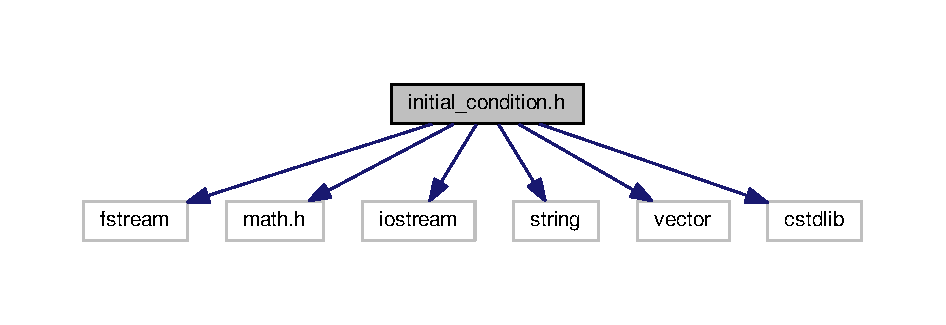
\includegraphics[width=350pt]{initial__condition_8h__incl}
\end{center}
\end{figure}
This graph shows which files directly or indirectly include this file\+:
\nopagebreak
\begin{figure}[H]
\begin{center}
\leavevmode
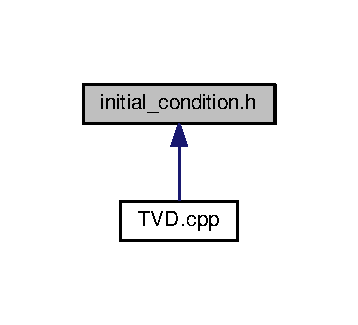
\includegraphics[width=172pt]{initial__condition_8h__dep__incl}
\end{center}
\end{figure}
\subsection*{Macros}
\begin{DoxyCompactItemize}
\item 
\#define \hyperlink{initial__condition_8h_ab683b1fef77e9bd4205b818c943fec96}{Specific\+Heat\+Ratio}~1.\+4
\item 
\#define \hyperlink{initial__condition_8h_ae9b1a60477a77e34837908fb3420118f}{Ideal\+Gas\+Constant}~287.\+14
\end{DoxyCompactItemize}
\subsection*{Functions}
\begin{DoxyCompactItemize}
\item 
double \hyperlink{initial__condition_8h_aacdb3b29cdea63bd2c4546c975d7370b}{find\+\_\+throat\+\_\+area} (std\+::vector$<$ std\+::vector$<$ double $>$ $>$ Upper\+Coordinates, int \&throat\+\_\+location)
\begin{DoxyCompactList}\small\item\em Function find\+\_\+throat() Finds the location of the throat. \end{DoxyCompactList}\item 
double \hyperlink{initial__condition_8h_aa49e9b4061bb2f4c566d4157723ca254}{get\+Mach} (double area\+Ratio)\hypertarget{initial__condition_8h_aa49e9b4061bb2f4c566d4157723ca254}{}\label{initial__condition_8h_aa49e9b4061bb2f4c566d4157723ca254}

\begin{DoxyCompactList}\small\item\em Function \hyperlink{initial__condition_8h_aa49e9b4061bb2f4c566d4157723ca254}{get\+Mach()} Finds the local Mach number for a given area ratio. \end{DoxyCompactList}\item 
double \hyperlink{initial__condition_8h_a3954c41c7a67bc08d0bb137807b49e6f}{get\+Area\+Ratio} (double Mach)\hypertarget{initial__condition_8h_a3954c41c7a67bc08d0bb137807b49e6f}{}\label{initial__condition_8h_a3954c41c7a67bc08d0bb137807b49e6f}

\begin{DoxyCompactList}\small\item\em Function \hyperlink{initial__condition_8h_a3954c41c7a67bc08d0bb137807b49e6f}{get\+Area\+Ratio()} Finds the area ratio for a given local Mach number. \end{DoxyCompactList}\item 
void \hyperlink{initial__condition_8h_a278f0d06446181043a0796e5e77ccc44}{initial\+\_\+condition} (vector$<$ vector$<$ vector$<$ vector$<$ double $>$ $>$ $>$ $>$ \&Conserved\+Variables, vector$<$ vector$<$ vector$<$ vector$<$ double $>$ $>$ $>$ $>$ \&Conserved\+Variables\+New, int Ni, int Nj, int Nk, int initial\+\_\+condition)
\begin{DoxyCompactList}\small\item\em Function \hyperlink{initial__condition_8h_a278f0d06446181043a0796e5e77ccc44}{initial\+\_\+condition()} \end{DoxyCompactList}\end{DoxyCompactItemize}


\subsection{Detailed Description}
This header file all conserved parameters inside the domain. Cureently, there are three different ways to do this. Use the appropriate switch statement. 

This header file all conserved parameters inside the domain.

\begin{DoxyAuthor}{Author}
Kuldeep Singh 
\end{DoxyAuthor}
\begin{DoxyDate}{Date}
2017
\end{DoxyDate}
\begin{DoxyAuthor}{Author}
Kuldeep Singh 
\end{DoxyAuthor}
\begin{DoxyDate}{Date}
2015 
\end{DoxyDate}


\subsection{Macro Definition Documentation}
\index{initial\+\_\+condition.\+h@{initial\+\_\+condition.\+h}!Ideal\+Gas\+Constant@{Ideal\+Gas\+Constant}}
\index{Ideal\+Gas\+Constant@{Ideal\+Gas\+Constant}!initial\+\_\+condition.\+h@{initial\+\_\+condition.\+h}}
\subsubsection[{\texorpdfstring{Ideal\+Gas\+Constant}{IdealGasConstant}}]{\setlength{\rightskip}{0pt plus 5cm}\#define Ideal\+Gas\+Constant~287.\+14}\hypertarget{initial__condition_8h_ae9b1a60477a77e34837908fb3420118f}{}\label{initial__condition_8h_ae9b1a60477a77e34837908fb3420118f}
This is ideal gas constant $ R(J Kg^{-1}K^{-1}) = (c_p - c_v)$ \index{initial\+\_\+condition.\+h@{initial\+\_\+condition.\+h}!Specific\+Heat\+Ratio@{Specific\+Heat\+Ratio}}
\index{Specific\+Heat\+Ratio@{Specific\+Heat\+Ratio}!initial\+\_\+condition.\+h@{initial\+\_\+condition.\+h}}
\subsubsection[{\texorpdfstring{Specific\+Heat\+Ratio}{SpecificHeatRatio}}]{\setlength{\rightskip}{0pt plus 5cm}\#define Specific\+Heat\+Ratio~1.\+4}\hypertarget{initial__condition_8h_ab683b1fef77e9bd4205b818c943fec96}{}\label{initial__condition_8h_ab683b1fef77e9bd4205b818c943fec96}
This is gas constant (Gamma). For air at room temperature it is almost equal to 1.\+4. If you are using some other gas at some other temperature then change it 

\subsection{Function Documentation}
\index{initial\+\_\+condition.\+h@{initial\+\_\+condition.\+h}!find\+\_\+throat\+\_\+area@{find\+\_\+throat\+\_\+area}}
\index{find\+\_\+throat\+\_\+area@{find\+\_\+throat\+\_\+area}!initial\+\_\+condition.\+h@{initial\+\_\+condition.\+h}}
\subsubsection[{\texorpdfstring{find\+\_\+throat\+\_\+area(std\+::vector$<$ std\+::vector$<$ double $>$ $>$ Upper\+Coordinates, int \&throat\+\_\+location)}{find_throat_area(std::vector< std::vector< double > > UpperCoordinates, int &throat_location)}}]{\setlength{\rightskip}{0pt plus 5cm}double find\+\_\+throat\+\_\+area (
\begin{DoxyParamCaption}
\item[{std\+::vector$<$ std\+::vector$<$ double $>$ $>$}]{Upper\+Coordinates, }
\item[{int \&}]{throat\+\_\+location}
\end{DoxyParamCaption}
)}\hypertarget{initial__condition_8h_aacdb3b29cdea63bd2c4546c975d7370b}{}\label{initial__condition_8h_aacdb3b29cdea63bd2c4546c975d7370b}


Function find\+\_\+throat() Finds the location of the throat. 


\begin{DoxyParams}{Parameters}
{\em throat\+\_\+area} & Area of the throat \\
\hline
\end{DoxyParams}
\index{initial\+\_\+condition.\+h@{initial\+\_\+condition.\+h}!initial\+\_\+condition@{initial\+\_\+condition}}
\index{initial\+\_\+condition@{initial\+\_\+condition}!initial\+\_\+condition.\+h@{initial\+\_\+condition.\+h}}
\subsubsection[{\texorpdfstring{initial\+\_\+condition(vector$<$ vector$<$ vector$<$ vector$<$ double $>$ $>$ $>$ $>$ \&\+Conserved\+Variables, vector$<$ vector$<$ vector$<$ vector$<$ double $>$ $>$ $>$ $>$ \&\+Conserved\+Variables\+New, int Ni, int Nj, int Nk, int initial\+\_\+condition)}{initial_condition(vector< vector< vector< vector< double > > > > &ConservedVariables, vector< vector< vector< vector< double > > > > &ConservedVariablesNew, int Ni, int Nj, int Nk, int initial_condition)}}]{\setlength{\rightskip}{0pt plus 5cm}void initial\+\_\+condition (
\begin{DoxyParamCaption}
\item[{vector$<$ vector$<$ vector$<$ vector$<$ double $>$ $>$ $>$ $>$ \&}]{Conserved\+Variables, }
\item[{vector$<$ vector$<$ vector$<$ vector$<$ double $>$ $>$ $>$ $>$ \&}]{Conserved\+Variables\+New, }
\item[{int}]{Ni, }
\item[{int}]{Nj, }
\item[{int}]{Nk, }
\item[{int}]{initial\+\_\+condition}
\end{DoxyParamCaption}
)}\hypertarget{initial__condition_8h_a278f0d06446181043a0796e5e77ccc44}{}\label{initial__condition_8h_a278f0d06446181043a0796e5e77ccc44}


Function \hyperlink{initial__condition_8h_a278f0d06446181043a0796e5e77ccc44}{initial\+\_\+condition()} 


\begin{DoxyParams}[1]{Parameters}
\mbox{\tt in}  & {\em Conserved\+Variables} & This is the pointer to the 4D vector where all the conserved variables of previous time step are stored. \\
\hline
\mbox{\tt in}  & {\em Conserved\+Variables\+New} & This is the pointer to the 4D vector where all the conserved variables of next/new time step are stored. \\
\hline
\mbox{\tt in}  & {\em Ni} & Number of cells in in \char`\"{}i\char`\"{} direction. \\
\hline
\mbox{\tt in}  & {\em Nj} & Number of cells in in \char`\"{}j\char`\"{} direction. \\
\hline
\mbox{\tt in}  & {\em Nk} & Number of cells in in \char`\"{}k\char`\"{} direction. \\
\hline
\end{DoxyParams}
\begin{DoxyReturn}{Returns}
void 
\end{DoxyReturn}
throat\+\_\+location Location of the throat


\begin{DoxyParams}{Parameters}
{\em throat\+\_\+area} & Area at the throat\\
\hline
{\em local\+\_\+area\+\_\+ratio} & Area ratio at a location with throat area\\
\hline
{\em Mach} & Mach number at a location\\
\hline
\end{DoxyParams}
Inlet conditions are user given data. one has to mention the stagnation parameters at inlet (ex. stagnation pressure ( $ P_0 $), temperature( $ T_0 $))


\begin{DoxyParams}{Parameters}
{\em Temperature\+Stagnation} & Stagnation temperature at inlet\\
\hline
{\em Pressure\+Stagnation} & Stagnation pressure at inlet\\
\hline
{\em Density\+Stagnation} & Stagnation density at inlet \\
\hline
\end{DoxyParams}

\hypertarget{interface_8h}{}\section{interface.\+h File Reference}
\label{interface_8h}\index{interface.\+h@{interface.\+h}}


This class calculates the interface parameters using Reo scheme flux.  


{\ttfamily \#include \char`\"{}math.\+h\char`\"{}}\\*
{\ttfamily \#include \char`\"{}iostream\char`\"{}}\\*
Include dependency graph for interface.\+h\+:\nopagebreak
\begin{figure}[H]
\begin{center}
\leavevmode
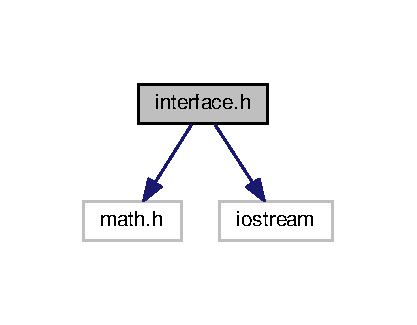
\includegraphics[width=200pt]{interface_8h__incl}
\end{center}
\end{figure}
This graph shows which files directly or indirectly include this file\+:
\nopagebreak
\begin{figure}[H]
\begin{center}
\leavevmode
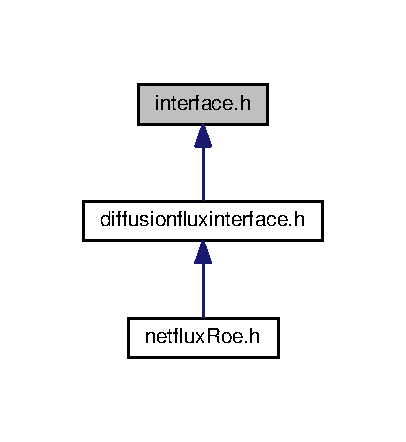
\includegraphics[width=199pt]{interface_8h__dep__incl}
\end{center}
\end{figure}
\subsection*{Classes}
\begin{DoxyCompactItemize}
\item 
class \hyperlink{classinterface}{interface}
\end{DoxyCompactItemize}
\subsection*{Macros}
\begin{DoxyCompactItemize}
\item 
\#define \hyperlink{interface_8h_ab683b1fef77e9bd4205b818c943fec96}{Specific\+Heat\+Ratio}~1.\+4
\end{DoxyCompactItemize}


\subsection{Detailed Description}
This class calculates the interface parameters using Reo scheme flux. 

\begin{DoxyAuthor}{Author}
Kuldeep Singh 
\end{DoxyAuthor}
\begin{DoxyDate}{Date}
2017 
\end{DoxyDate}
\begin{DoxyCopyright}{Copyright}
G\+NU Public License. 
\end{DoxyCopyright}

\begin{DoxyParams}[1]{Parameters}
 & {\em Density\+Interface} & Roe density at interface \\
\hline
 & {\em Velocity\+X\+Interface} & x velocity at interface \\
\hline
 & {\em Velocity\+Y\+Interface} & y velocity at interface \\
\hline
 & {\em Velocity\+Z\+Interface} & z velocity at interface \\
\hline
 & {\em Enthalpy\+Interface} & Enthalpy at interface \\
\hline
 & {\em Enthalpy\+Interface} & Enthalpy at interface \\
\hline
 & {\em Vector\+Jump\+Interface} & Change in the conserved parameters at the interface \\
\hline
 & {\em Eigen\+Value} & Eigenvalue of the Jacobian matrix \\
\hline
 & {\em Eigen\+Vector\+Matrix} & Eigenvector of the Jacobian matrix \\
\hline
 & {\em Eigen\+Vector\+Matrix\+Inverse} & Inverse of the Jacobian matrix \\
\hline
 & {\em Alpha\+Vector\+Interface\mbox{[}5\mbox{]}} & Eigen\+Vector\+Matrix\+Inverse\mbox{[}5\mbox{]}\mbox{[}5\mbox{]}$\ast$\+Vector\+Jump\+Interface \\
\hline
 & {\em Mu\+Vector\+Interface} & = delta t $\ast$ Eigen\+Value \\
\hline
 & {\em Z\+Vector\+Interface} & This is same as Mu\+Vector\+Interface \\
\hline
\mbox{\tt in}  & {\em Conserved\+Variables} & This is the pointer to the 4D vector where all the conserved variables of previous time step are stored. \\
\hline
\mbox{\tt in}  & {\em Face\+Area\+Vector\+Interface} & This is the pointer to the area vector the cell interface \\
\hline
 & {\em Cell\+Volume} & 3D vector which has the cell volume of all cells inside the domain \\
\hline
\end{DoxyParams}


\subsection{Macro Definition Documentation}
\index{interface.\+h@{interface.\+h}!Specific\+Heat\+Ratio@{Specific\+Heat\+Ratio}}
\index{Specific\+Heat\+Ratio@{Specific\+Heat\+Ratio}!interface.\+h@{interface.\+h}}
\subsubsection[{\texorpdfstring{Specific\+Heat\+Ratio}{SpecificHeatRatio}}]{\setlength{\rightskip}{0pt plus 5cm}\#define Specific\+Heat\+Ratio~1.\+4}\hypertarget{interface_8h_ab683b1fef77e9bd4205b818c943fec96}{}\label{interface_8h_ab683b1fef77e9bd4205b818c943fec96}
This is gas constant (Gamma). For air at room temperature it is almost equal to 1.\+4. If you are using some other gas at some other temperature then change it 
\hypertarget{local__time__step_8h}{}\section{local\+\_\+time\+\_\+step.\+h File Reference}
\label{local__time__step_8h}\index{local\+\_\+time\+\_\+step.\+h@{local\+\_\+time\+\_\+step.\+h}}


This header file conditions the function Time\+Step() which calculate the local time step for each cell at every iteration.  


{\ttfamily \#include $<$vector$>$}\\*
{\ttfamily \#include $<$math.\+h$>$}\\*
Include dependency graph for local\+\_\+time\+\_\+step.\+h\+:\nopagebreak
\begin{figure}[H]
\begin{center}
\leavevmode
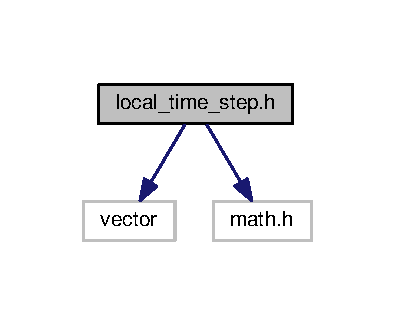
\includegraphics[width=190pt]{local__time__step_8h__incl}
\end{center}
\end{figure}
\subsection*{Functions}
\begin{DoxyCompactItemize}
\item 
double {\bfseries Time\+Step} (int i, int j, int k, vector$<$ vector$<$ vector$<$ double $>$ $>$ $>$ delta\+\_\+s, vector$<$ vector$<$ vector$<$ vector$<$ double $>$ $>$ $>$ $>$ Conserved\+Variables)\hypertarget{local__time__step_8h_a9a9d3b47de7cb00d45159818b69d0843}{}\label{local__time__step_8h_a9a9d3b47de7cb00d45159818b69d0843}

\end{DoxyCompactItemize}


\subsection{Detailed Description}
This header file conditions the function Time\+Step() which calculate the local time step for each cell at every iteration. 

\begin{DoxyAuthor}{Author}
Kuldeep Singh 
\end{DoxyAuthor}
\begin{DoxyDate}{Date}
2016 
\end{DoxyDate}
\begin{DoxySeeAlso}{See also}
\hyperlink{grid__ideal__nozzle_8h_a0195a06d59a6445d9ef8d27b775caeb0}{grid()} 
\end{DoxySeeAlso}
\begin{DoxyRefDesc}{Bug}
\item[\hyperlink{bug__bug000007}{Bug}]Currently not using this, because \hyperlink{grid__ideal__nozzle_8h_a0195a06d59a6445d9ef8d27b775caeb0}{grid()} is not calculating ds value. So recheck this function as well after fixing the \hyperlink{grid__ideal__nozzle_8h_a0195a06d59a6445d9ef8d27b775caeb0}{grid()} function. \end{DoxyRefDesc}

\begin{DoxyParams}[1]{Parameters}
\mbox{\tt in}  & {\em i,j,k} & Cell location for which Time\+Step is to be calculated \\
\hline
\mbox{\tt in}  & {\em delta\+\_\+s} & ds value of the cell for which Time\+Step is to be calculated \\
\hline
 & {\em \mbox{[}\+I\+N\mbox{]}} & Conserved\+Variables Conserved variables vector \\
\hline
 & {\em C\+FL} & Courant–\+Friedrichs–\+Lewy number \\
\hline
 & {\em Pressure} & Static Pressure \\
\hline
 & {\em Velocity\+Magnitude} & Magnitude of the velocity \\
\hline
 & {\em Velocity\+Sound} & Speed of sound \\
\hline
\mbox{\tt out}  & {\em Time\+Step} & Time step (dt) \\
\hline
\end{DoxyParams}
\begin{DoxyReturn}{Returns}
double 
\end{DoxyReturn}

\hypertarget{netfluxinterface_8h}{}\section{netfluxinterface.\+h File Reference}
\label{netfluxinterface_8h}\index{netfluxinterface.\+h@{netfluxinterface.\+h}}


Calculates the net flux vector(numerical diffusion and euler flux) at the interface.  


{\ttfamily \#include \char`\"{}math.\+h\char`\"{}}\\*
{\ttfamily \#include \char`\"{}eulerflux.\+h\char`\"{}}\\*
{\ttfamily \#include \char`\"{}diffusionfluxinterface.\+h\char`\"{}}\\*
Include dependency graph for netfluxinterface.\+h\+:
% FIG 0
This graph shows which files directly or indirectly include this file\+:
% FIG 1
\subsection*{Classes}
\begin{DoxyCompactItemize}
\item 
class \hyperlink{classnetfluxinterface}{netfluxinterface}
\end{DoxyCompactItemize}


\subsection{Detailed Description}
Calculates the net flux vector(numerical diffusion and euler flux) at the interface. 

This class uses the two other class. One Euler for euler fulx calculation and second for numerical diffusion flux calculation. \begin{DoxyAuthor}{Author}
Kuldeep Singh 
\end{DoxyAuthor}
\begin{DoxyDate}{Date}
2015 
\end{DoxyDate}
\begin{DoxyCopyright}{Copyright}
G\+NU Public License(\+G\+P\+L). 
\end{DoxyCopyright}

\hypertarget{TVD_8cpp}{}\section{T\+V\+D.\+cpp File Reference}
\label{TVD_8cpp}\index{T\+V\+D.\+cpp@{T\+V\+D.\+cpp}}


This header file contains the run() function which runs the solver.  


{\ttfamily \#include \char`\"{}iostream\char`\"{}}\\*
{\ttfamily \#include $<$vector$>$}\\*
{\ttfamily \#include $<$fstream$>$}\\*
{\ttfamily \#include \char`\"{}math.\+h\char`\"{}}\\*
{\ttfamily \#include \char`\"{}time.\+h\char`\"{}}\\*
{\ttfamily \#include \char`\"{}netfluxinterface.\+h\char`\"{}}\\*
{\ttfamily \#include \char`\"{}grid\+\_\+nozzle.\+h\char`\"{}}\\*
{\ttfamily \#include \char`\"{}B\+C.\+h\char`\"{}}\\*
Include dependency graph for T\+V\+D.\+cpp\+:
\nopagebreak
\begin{figure}[H]
\begin{center}
\leavevmode
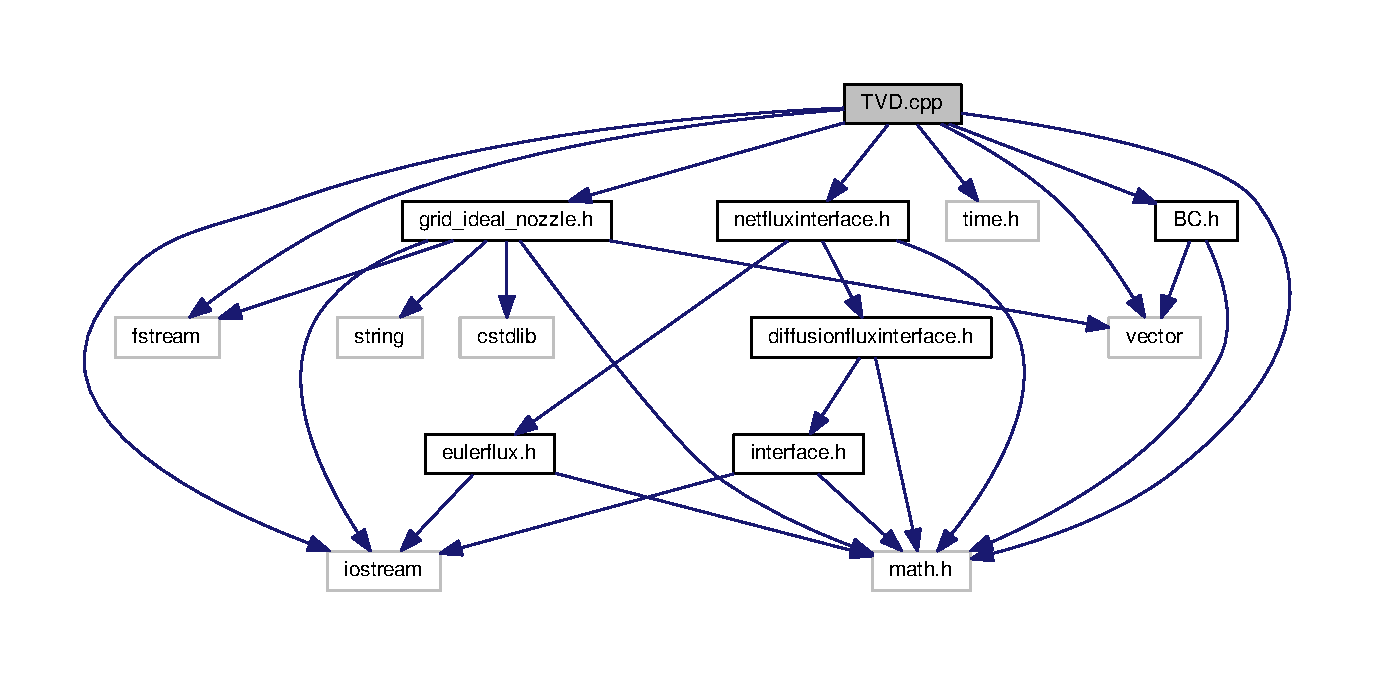
\includegraphics[width=350pt]{TVD_8cpp__incl}
\end{center}
\end{figure}
\subsection*{Functions}
\begin{DoxyCompactItemize}
\item 
void \hyperlink{TVD_8cpp_aceceec12d8564f6adae5642b12db51fe}{BC} (vector$<$ vector$<$ vector$<$ vector$<$ double $>$ $>$ $>$ $>$ \&Conserved\+Variables, vector$<$ vector$<$ vector$<$ vector$<$ double $>$ $>$ $>$ $>$ \&j\+Face\+Area\+Vector, vector$<$ vector$<$ vector$<$ vector$<$ double $>$ $>$ $>$ $>$ \&k\+Face\+Area\+Vector, int Ni, int Nj, int Nk)
\begin{DoxyCompactList}\small\item\em This function implements the boundary condition, i\+Face\+Area\+Vector is not required Because currently the flow in x direction and 2D flow. \end{DoxyCompactList}\item 
void \hyperlink{TVD_8cpp_ac7609273a01eb63ff8a25ddf1aafeff7}{grid} (vector$<$ vector$<$ vector$<$ vector$<$ double $>$ $>$ $>$ $>$ \&i\+Face\+Area\+Vector, vector$<$ vector$<$ vector$<$ vector$<$ double $>$ $>$ $>$ $>$ \&j\+Face\+Area\+Vector, vector$<$ vector$<$ vector$<$ vector$<$ double $>$ $>$ $>$ $>$ \&k\+Face\+Area\+Vector, vector$<$ vector$<$ vector$<$ double $>$ $>$ $>$ \&Cell\+Volume, vector$<$ vector$<$ vector$<$ double $>$ $>$ $>$ \&delta\+\_\+s, int \&Ni, int \&Nj, int \&Nk)
\begin{DoxyCompactList}\small\item\em This function generates the area vector and cell volumes inside the domain whole domain. \end{DoxyCompactList}\item 
int \hyperlink{TVD_8cpp_ae66f6b31b5ad750f1fe042a706a4e3d4}{main} ()
\begin{DoxyCompactList}\small\item\em This function runs the solver. \end{DoxyCompactList}\end{DoxyCompactItemize}


\subsection{Detailed Description}
This header file contains the run() function which runs the solver. 

\begin{DoxyAuthor}{Author}
Kuldeep Singh 
\end{DoxyAuthor}
\begin{DoxyDate}{Date}
2017 
\end{DoxyDate}


\subsection{Function Documentation}
\index{T\+V\+D.\+cpp@{T\+V\+D.\+cpp}!BC@{BC}}
\index{BC@{BC}!T\+V\+D.\+cpp@{T\+V\+D.\+cpp}}
\subsubsection[{\texorpdfstring{B\+C(vector$<$ vector$<$ vector$<$ vector$<$ double $>$ $>$ $>$ $>$ \&\+Conserved\+Variables, vector$<$ vector$<$ vector$<$ vector$<$ double $>$ $>$ $>$ $>$ \&j\+Face\+Area\+Vector, vector$<$ vector$<$ vector$<$ vector$<$ double $>$ $>$ $>$ $>$ \&k\+Face\+Area\+Vector, int Ni, int Nj, int Nk)}{BC(vector< vector< vector< vector< double > > > > &ConservedVariables, vector< vector< vector< vector< double > > > > &jFaceAreaVector, vector< vector< vector< vector< double > > > > &kFaceAreaVector, int Ni, int Nj, int Nk)}}]{\setlength{\rightskip}{0pt plus 5cm}void BC (
\begin{DoxyParamCaption}
\item[{vector$<$ vector$<$ vector$<$ vector$<$ double $>$ $>$ $>$ $>$ \&}]{Conserved\+Variables, }
\item[{vector$<$ vector$<$ vector$<$ vector$<$ double $>$ $>$ $>$ $>$ \&}]{j\+Face\+Area\+Vector, }
\item[{vector$<$ vector$<$ vector$<$ vector$<$ double $>$ $>$ $>$ $>$ \&}]{k\+Face\+Area\+Vector, }
\item[{int}]{Ni, }
\item[{int}]{Nj, }
\item[{int}]{Nk}
\end{DoxyParamCaption}
)}\hypertarget{TVD_8cpp_aceceec12d8564f6adae5642b12db51fe}{}\label{TVD_8cpp_aceceec12d8564f6adae5642b12db51fe}


This function implements the boundary condition, i\+Face\+Area\+Vector is not required Because currently the flow in x direction and 2D flow. 

This function implements the boundary condition, i\+Face\+Area\+Vector is not required Because currently the flow in x direction and 2D flow.


\begin{DoxyParams}[1]{Parameters}
\mbox{\tt in}  & {\em Conserved\+Variables} & This is the pointer to the 4D vector where all the conserved variables of previous time step are stored. \\
\hline
\mbox{\tt in}  & {\em \&i\+Face\+Area\+Vector} & This is a pointer to the 4D vector which has the area vector of all faces which are in \char`\"{}i\char`\"{} direction. \\
\hline
\mbox{\tt in}  & {\em \&j\+Face\+Area\+Vector} & This is a pointer to the 4D vector which has the area vector of all faces which are in \char`\"{}j\char`\"{} direction. \\
\hline
\mbox{\tt in}  & {\em \&k\+Face\+Area\+Vector} & This is a pointer to the 4D vector which has the area vector of all faces which are in \char`\"{}k\char`\"{} direction. \\
\hline
\mbox{\tt in}  & {\em Ni} & Number of cells in in \char`\"{}i\char`\"{} direction. \\
\hline
\mbox{\tt in}  & {\em Nj} & Number of cells in in \char`\"{}j\char`\"{} direction. \\
\hline
\mbox{\tt in}  & {\em Nk} & Number of cells in in \char`\"{}k\char`\"{} direction. \\
\hline
\end{DoxyParams}
\begin{DoxyReturn}{Returns}
void 
\end{DoxyReturn}
Inlet conditions are user given data. one has to mention the stagnation parameters at inlet (ex. stagnation pressure ( $ P_0 $), temperature( $ T_0 $))


\begin{DoxyParams}{Parameters}
{\em Temperature\+Stagnation} & Stagnation temperature at inlet\\
\hline
{\em Pressure\+Stagnation} & Stagnation pressure at inlet\\
\hline
{\em Density\+Stagnation} & Stagnation density at inlet\\
\hline
{\em Geometry} & rotation angle\\
\hline
{\em Inlet\+Pressure} & Static pressure at inlet\\
\hline
{\em Mach} & Mach number at inlet\\
\hline
{\em Inlet\+Temperature} & Static temperature at inlet\\
\hline
{\em Inlet\+Velocity} & Flow velocity at inlet\\
\hline
{\em Inlet\+Density} & Flow density at inlet \\
\hline
\end{DoxyParams}
\index{T\+V\+D.\+cpp@{T\+V\+D.\+cpp}!grid@{grid}}
\index{grid@{grid}!T\+V\+D.\+cpp@{T\+V\+D.\+cpp}}
\subsubsection[{\texorpdfstring{grid(vector$<$ vector$<$ vector$<$ vector$<$ double $>$ $>$ $>$ $>$ \&i\+Face\+Area\+Vector, vector$<$ vector$<$ vector$<$ vector$<$ double $>$ $>$ $>$ $>$ \&j\+Face\+Area\+Vector, vector$<$ vector$<$ vector$<$ vector$<$ double $>$ $>$ $>$ $>$ \&k\+Face\+Area\+Vector, vector$<$ vector$<$ vector$<$ double $>$ $>$ $>$ \&\+Cell\+Volume, vector$<$ vector$<$ vector$<$ double $>$ $>$ $>$ \&delta\+\_\+s, int \&\+Ni, int \&\+Nj, int \&\+Nk)}{grid(vector< vector< vector< vector< double > > > > &iFaceAreaVector, vector< vector< vector< vector< double > > > > &jFaceAreaVector, vector< vector< vector< vector< double > > > > &kFaceAreaVector, vector< vector< vector< double > > > &CellVolume, vector< vector< vector< double > > > &delta_s, int &Ni, int &Nj, int &Nk)}}]{\setlength{\rightskip}{0pt plus 5cm}void grid (
\begin{DoxyParamCaption}
\item[{vector$<$ vector$<$ vector$<$ vector$<$ double $>$ $>$ $>$ $>$ \&}]{i\+Face\+Area\+Vector\+In, }
\item[{vector$<$ vector$<$ vector$<$ vector$<$ double $>$ $>$ $>$ $>$ \&}]{j\+Face\+Area\+Vector\+In, }
\item[{vector$<$ vector$<$ vector$<$ vector$<$ double $>$ $>$ $>$ $>$ \&}]{k\+Face\+Area\+Vector\+In, }
\item[{vector$<$ vector$<$ vector$<$ double $>$ $>$ $>$ \&}]{Cell\+Volume\+In, }
\item[{vector$<$ vector$<$ vector$<$ double $>$ $>$ $>$ \&}]{ds\+In, }
\item[{int \&}]{Ni, }
\item[{int \&}]{Nj, }
\item[{int \&}]{Nk}
\end{DoxyParamCaption}
)}\hypertarget{TVD_8cpp_ac7609273a01eb63ff8a25ddf1aafeff7}{}\label{TVD_8cpp_ac7609273a01eb63ff8a25ddf1aafeff7}


This function generates the area vector and cell volumes inside the domain whole domain. 

This function generates the area vector and cell volumes inside the domain whole domain.


\begin{DoxyParams}[1]{Parameters}
\mbox{\tt in}  & {\em i\+Face\+Area\+Vector\+In} & Input pointer to \char`\"{}i\char`\"{} faces area vector \\
\hline
\mbox{\tt in}  & {\em j\+Face\+Area\+Vector\+In} & Input pointer to \char`\"{}j\char`\"{} faces area vector \\
\hline
\mbox{\tt in}  & {\em k\+Face\+Area\+Vector\+In} & Input pointer to \char`\"{}k\char`\"{} faces area vector \\
\hline
\mbox{\tt in}  & {\em Cell\+Volume\+In} & Input pointer to cell volumes \\
\hline
\mbox{\tt in}  & {\em ds\+In} & Input pointer to minimum distance \\
\hline
 & {\em Upper\+Coordinates} & Upper wall coordinates (x,y) of the nozzle geometry \\
\hline
 & {\em Down\+Coordinates} & Down wall coordinates (x,y) of the nozzle geometry \\
\hline
\end{DoxyParams}
\begin{DoxyReturn}{Returns}
void 
\end{DoxyReturn}

\begin{DoxyParams}[1]{Parameters}
 & {\em N} & Total cells in j direction\\
\hline
 & {\em N+1} & Total grid points in j direction after including the boundary points\\
\hline
\mbox{\tt in}  & {\em Ni} & Input number of cells in in \char`\"{}i\char`\"{} direction.\\
\hline
\mbox{\tt in}  & {\em Nj} & Input number of cells in in \char`\"{}j\char`\"{} direction.\\
\hline
\mbox{\tt in}  & {\em Nk} & Input number of cells in in \char`\"{}k\char`\"{} direction.\\
\hline
 & {\em Coordinate} & 4D vector which stores the all coordinates of all cells inside the domain\\
\hline
 & {\em i\+Face\+Area\+Vector} & 4D vector which stores the all \char`\"{}i\char`\"{} face area vectors of all cells inside the domain\\
\hline
 & {\em j\+Face\+Area\+Vector} & 4D vector which stores the all \char`\"{}j\char`\"{} face area vectors of all cells inside the domain\\
\hline
 & {\em k\+Face\+Area\+Vector} & 4D vector which stores the all \char`\"{}k\char`\"{} face area vectors of all cells inside the domain\\
\hline
 & {\em Cell\+Volume} & 3D vector which stores the cell volume of all cells inside the domain\\
\hline
 & {\em (x0,y0)} & Live cell coordinates which needs to be mirrored to get the ghost cell coordinates\\
\hline
 & {\em (x1,y1)} & Next live cell coordinates which needs to be mirrored to get the ghost cell coordinates\\
\hline
 & {\em (l0,m0),(l1,m1)} & Line about which reflection needs to be taken\\
\hline
 & {\em (rx0,ry0)} & Ghost cell grid point\\
\hline
 & {\em (rx1,ry1)} & Ghost cell next grid point\\
\hline
\end{DoxyParams}
\begin{DoxyRefDesc}{Bug}
\item[\hyperlink{bug__bug000006}{Bug}]Yet to calculate the ds value properly \end{DoxyRefDesc}


Structure of grid out put file (\char`\"{}grids\+\_\+\+Nozzle\+\_\+2\+D.\+csv\char`\"{})
\begin{DoxyItemize}
\item First line of the grid file will contain grid points (excluding ghost cells) in x and y direction
\item This will exclude the ghost, only live cells or actual geomatry points
\end{DoxyItemize}\index{T\+V\+D.\+cpp@{T\+V\+D.\+cpp}!main@{main}}
\index{main@{main}!T\+V\+D.\+cpp@{T\+V\+D.\+cpp}}
\subsubsection[{\texorpdfstring{main()}{main()}}]{\setlength{\rightskip}{0pt plus 5cm}int main (
\begin{DoxyParamCaption}
{}
\end{DoxyParamCaption}
)}\hypertarget{TVD_8cpp_ae66f6b31b5ad750f1fe042a706a4e3d4}{}\label{TVD_8cpp_ae66f6b31b5ad750f1fe042a706a4e3d4}


This function runs the solver. 

\begin{DoxyWarning}{Warning}
Currently not using this, because \hyperlink{TVD_8cpp_ac7609273a01eb63ff8a25ddf1aafeff7}{grid()} is not calculating ds value properly. So recheck this function as well after fixing the \hyperlink{TVD_8cpp_ac7609273a01eb63ff8a25ddf1aafeff7}{grid()} function. 
\end{DoxyWarning}
\begin{DoxyReturn}{Returns}
double 
\end{DoxyReturn}

\begin{DoxyParams}{Parameters}
{\em Start\+Time} & Simulation starting time\\
\hline
{\em End\+Time} & Simulation ending time\\
\hline
{\em DeltaT} & Time step\\
\hline
{\em Iteration\+Values} & Total iterations = floor(T\+I\+M\+E/\+DeltaT)\\
\hline
{\em Ni} & Number of cells in in \char`\"{}i\char`\"{} direction.\\
\hline
{\em Nj} & Number of cells in in \char`\"{}j\char`\"{} direction.\\
\hline
{\em Nk} & Number of cells in in \char`\"{}k\char`\"{} direction.\\
\hline
{\em \&i\+Face\+Area\+Vector} & This is a pointer to the 4D vector which has the area vector of all faces which are in \char`\"{}i\char`\"{} direction.\\
\hline
{\em \&j\+Face\+Area\+Vector} & This is a pointer to the 4D vector which has the area vector of all faces which are in \char`\"{}j\char`\"{} direction.\\
\hline
{\em \&k\+Face\+Area\+Vector} & This is a pointer to the 4D vector which has the area vector of all faces which are in \char`\"{}k\char`\"{} direction.\\
\hline
{\em Cell\+Volume\+In} & Input pointer to cell volumes\\
\hline
{\em delta\+\_\+s} & Minimum distance\\
\hline
{\em Conserved\+Variables} & This is the pointer to the 4D vector where all the conserved variables (\mbox{[}Density , x-\/momentum, y-\/momentum, z-\/momentum, Energy\mbox{]}) of previous time step are stored.\\
\hline
{\em Conserved\+Variables\+New} & This is the pointer to the 4D vector where all the conserved variables (\mbox{[}Density , x-\/momentum, y-\/momentum, z-\/momentum, Energy\mbox{]}) of current/new time step are stored.\\
\hline
\end{DoxyParams}
\begin{DoxyRefDesc}{Bug}
\item[\hyperlink{bug__bug000009}{Bug}]Every time simulation starts from first iteration. So, to save the simulation it is good to start from the last solution as the initial condition \end{DoxyRefDesc}



\begin{DoxyParams}{Parameters}
{\em i\+Cell\+Interface\+Volume} & Average of right and left cell volume in i direction\\
\hline
{\em j\+Cell\+Interface\+Volume} & Average of right and left cell volume in j direction\\
\hline
{\em k\+Cell\+Interface\+Volume} & Average of right and left cell volume in k direction\\
\hline
\end{DoxyParams}
\begin{DoxyRefDesc}{Bug}
\item[\hyperlink{bug__bug000010}{Bug}]Local time step needs to be used to reduce the simulation time \end{DoxyRefDesc}



\begin{DoxyParams}{Parameters}
{\em Density\+Residual} & Density residual\\
\hline
{\em x\+Momentum\+Residual} & x Momentum residual\\
\hline
{\em y\+Momentum\+Residual} & y Momentum residual\\
\hline
{\em z\+Momentum\+Residual} & z Momentum residual\\
\hline
{\em Energy} & residual\\
\hline
{\em } & \\
\hline
\end{DoxyParams}

%--- End generated contents ---

% Index
\backmatter
\newpage
\phantomsection
\clearemptydoublepage
\addcontentsline{toc}{chapter}{Index}
\printindex

\end{document}
